%Version 4.0 Revised - Systems Paper with All Figures
%Summary of Major Changes:
%- Added all professional architecture diagrams
%- Added actual UI screenshots from the system
%- Added complexity analysis table
%- Added LangChain integration details
%- Added validation heatmap (illustrative)
%- Professional black/white diagram style
%- Included analytics visualizations

\documentclass[11pt]{article}

%%%% Standard Packages
\usepackage[top=1in, bottom=1in, left=1in, right=1in]{geometry}
\usepackage{graphicx}
\usepackage{multirow}
\usepackage{amsmath,amssymb,amsfonts}
\usepackage{amsthm}
\usepackage{mathrsfs}
\usepackage[title]{appendix}
\usepackage{xcolor}
\usepackage{textcomp}
\usepackage{booktabs}
\usepackage{algorithm}
\usepackage{algorithmicx}
\usepackage{algpseudocode}
\usepackage{listings}
\usepackage{float}
\usepackage{array}
\usepackage{enumitem}
\usepackage{hyperref}

\hypersetup{
    colorlinks=true,
    linkcolor=blue,
    urlcolor=blue,
    citecolor=blue
}

\raggedbottom

\title{Beyond Difficulty Scaling: Simulating Learning Disabilities with LLM-Powered Visual Analytics}

\author{
Atharv Raotole$^{1}$ \and Vishnu Sai Kotha$^{2}$ \and Anaya Patel$^{2}$ \and Klaus Mueller$^{3}$ \\
$^{1}$Department of Data Science, Stony Brook University \\
$^{2}$Department of Computer Science, Stony Brook University \\
$^{3}$Department of Computer Science, Stony Brook University \\
\texttt{\{atharv.raotole, vishnu.kotha, anaya.patel\}@stonybrook.edu}, \texttt{mueller@cs.stonybrook.edu}
}

\date{}

\begin{document}

\maketitle

\begin{abstract}
\noindent
Mathematics education faces a critical challenge: students with learning disabilities struggle to achieve proficiency because educational technologies oversimplify disability-specific cognitive patterns into difficulty-scaling problems. We present an LLM-powered visual analytics system that generates authentic disability-specific mathematical problem-solving simulations, providing educators with actionable, evidence-based teaching strategies.\footnote{An anonymized demo is available at: \url{https://clownfish-app-srrai.ondigitalocean.app/}} Our system integrates three technical innovations: (1) a LangGraph workflow architecture orchestrating problem generation, disability-specific simulation, cognitive analysis, and intervention recommendation through eight interconnected processing nodes; (2) a multi-dimensional validation framework with five orthogonal consistency metrics ensuring authentic representation of disability behaviors; and (3) a visual analytics dashboard enabling rapid assessment through temporal trend visualization and progressive disclosure. The system leverages LangChain for LLM integration with structured prompt engineering, implementing temperature-calibrated generation across workflow stages. Supporting seven disability types across grades 2--7, we validate the system through a pilot technical evaluation ($N=10$ sessions) demonstrating simulation authenticity ($\bar{\kappa}=0.84$), cognitive analysis precision, and practical latency under 15 seconds per session at approximately \$0.03 cost. This work serves as both a professional development tool and a research platform for understanding learning disability manifestations in mathematical cognition.
\end{abstract}

\textbf{Keywords:} Visual analytics, Learning disabilities, Educational visualization, Adaptive learning systems, Large language models, Special education technology

%-------------------------------------------------------------------------
\section{Introduction}\label{sec:intro}

Learning disabilities affect approximately 15\% of students worldwide~\cite{ref1}, yet educational systems continue to struggle with providing appropriate accommodations. Consider two students in a typical middle school mathematics class:

A fifth-grade student with dyscalculia stares at a multiplication problem involving fractions. She understands that the recipe requires scaling ingredients, but repeatedly adds the fractions instead of multiplying them. To her teacher, this looks like a ``careless mistake.'' In reality, it reflects a fundamental challenge with numerical operations: her brain consistently confuses operational symbols despite understanding the problem's context.

A seventh-grader with dyslexia reads ``Calculate 63 $\div$ 7'' but processes it as ``36 $\div$ 7.'' He sets up the long division carefully, shows his work methodically, and arrives at an incorrect answer. This happens not because he lacks division skills, but because symbol reversals transform a solvable problem into an impossible puzzle.

These are not simply ``careless mistakes.'' They represent fundamental differences in how students process mathematical information. Yet current educational technologies treat learning disabilities as a simple difficulty scaling problem: if a student struggles, reduce complexity. This oversimplification fails to address the nuanced ways different disabilities manifest in mathematical thinking. A student with ADHD might excel at conceptual understanding but lose focus during multi-step problems, while a student with dysgraphia might grasp the solution mentally but struggle to organize their written work. Generic accommodations cannot adequately support such diverse needs.

Recent advances in Large Language Models present an opportunity to transform this landscape. LLMs demonstrate remarkable capabilities in understanding context, generating human-like text, and reasoning about complex scenarios. However, their application to special education requires careful engineering to ensure authenticity, consistency, and educational validity. Simply prompting an LLM to ``act like a student with dyslexia'' produces unreliable results without proper constraints and validation mechanisms~\cite{ref11,ref12}.

We address these challenges through an integrated system combining LLM capabilities with structured workflow orchestration, rigorous validation frameworks, and evidence-based pedagogical principles.

\subsection{Our Contributions}\label{subsec:contributions}

Our contributions span technical innovation and educational impact:

\begin{enumerate}
    \item A \textbf{disability-specific simulation framework} generating authentic student responses reflecting how different learning disabilities manifest in mathematical problem-solving, grounded in parameterized disability profiles derived from special education literature.
    
    \item A \textbf{multi-dimensional consistency validation system} with five orthogonal metrics (step-answer consistency, disability-specific behavior, mathematical reasoning, error patterns, and completeness) designed to ensure simulated responses accurately reflect disability characteristics.
    
    \item A \textbf{visual analytics architecture} balancing comprehensive assessment with cognitive load management through temporal encoding, multi-dimensional visualization, and progressive disclosure principles.
    
    \item An \textbf{adaptive difficulty management algorithm} that analyzes performance history using trend coefficients and multi-threshold decision logic, moving beyond simple accuracy-based adjustments.
    
    \item A \textbf{comprehensive cognitive analysis pipeline} identifying specific error patterns and generating evidence-based teaching strategies through structured prompt engineering.
    
    \item \textbf{LangGraph workflow orchestration} with eight interconnected nodes enabling sophisticated multi-stage educational processing while maintaining modularity and extensibility.
    
    \item We formalize a multi-dimensional validation and adaptive difficulty framework and illustrate its use on realistic scenarios through detailed case studies.
\end{enumerate}

The system supports seven types of learning disabilities (Dyslexia, Dyscalculia, ADHD, Dysgraphia, Auditory Processing Disorder, Non-verbal Learning Disorder, and Language Processing Disorder) across grades 2--7 with three difficulty levels.

%-------------------------------------------------------------------------
\section{Related Work}\label{sec:related}

The challenge of supporting students with learning disabilities in mathematics sits at the intersection of special education pedagogy, adaptive learning systems, artificial intelligence in education, and visual analytics for teaching. While each domain has made significant strides independently, the synthesis of disability-specific cognitive modeling, teacher-centered tool design, and validated generative AI approaches remains largely unexplored.

Learning disabilities represent one of the most pressing challenges in modern education, affecting approximately 15\% of students worldwide with 7.5 million students receiving special education services in the U.S. alone~\cite{ref1}. The persistent achievement gap is stark: students with learning disabilities consistently fail to achieve mathematics proficiency~\cite{ref2}, a statistic that has remained stubbornly resistant to improvement despite decades of intervention research. Recent research has begun moving beyond simple ``right or wrong'' assessments toward more nuanced understanding of mathematical errors. Lin et al.~\cite{ref4} provide a comprehensive taxonomy classifying errors into conceptual misunderstandings, procedural mistakes, factual recall failures, and careless slips, each requiring fundamentally different instructional responses. Geary and vanMarle~\cite{ref6} extend this work by documenting how specific disabilities manifest distinctly in mathematical cognition: dyscalculia affects core number sense and numerical operations, while dyslexia primarily impacts symbol recognition and reading of mathematical notation. Butterworth et al.~\cite{ref7} demonstrate through neuroimaging studies that these differences reflect underlying neurological variations rather than simply different levels of mathematical ability.

The field of Intelligent Tutoring Systems (ITS) has long promised personalized learning experiences, yet traditional approaches face fundamental limitations when applied to learning disabilities. Son~\cite{ref9} and Zixiang~\cite{ref10} provide comprehensive reviews showing that most ITS rely on hand-crafted cognitive models, essentially elaborate rule systems encoding expert knowledge about common misconceptions and solution strategies. While effective for typical learners, these systems prove brittle when confronted with the diverse error patterns exhibited by students with disabilities. Computer Adaptive Testing systems using Item Response Theory (IRT) face similar challenges. Benton~\cite{ref11} argues that IRT's assumption of unidimensional ability becomes problematic when neurocognitive deficits introduce systematic biases that violate the model's mathematical foundations. VanLehn~\cite{ref12} demonstrates through meta-analysis that human tutors remain significantly more effective than automated systems, particularly for struggling learners, suggesting that current ITS miss something essential about adaptive human teaching.

The emergence of powerful Large Language Models has catalyzed a wave of educational technology research, though the landscape remains uneven. Kasneci et al.~\cite{ref16} observe that over 90\% of studies examining LLMs in education focus on ChatGPT applications in medical education and English language learning, leaving K--12 mathematics and special education significantly under-researched. Desmarais and Baker~\cite{ref15} provide a forward-looking perspective on bringing generative AI to adaptive learning, arguing that LLMs' ability to generate novel content and explanations could fundamentally transform educational technology. Wang et al.~\cite{ref18} explore using LLMs as student simulators for evaluating educational interventions, demonstrating that with appropriate prompting, language models can generate responses that human educators find realistic. Liu et al.~\cite{ref19} present a modular generative ITS architecture leveraging GPT-4, demonstrating how structured JSON outputs can enable systematic educational processing.

The visual analytics community has increasingly turned attention toward education. Mart\'inez-Maldonado et al.~\cite{ref24} present CADA, a teacher-facing learning analytics dashboard emphasizing actionable insights over raw metrics. Schwendimann et al.~\cite{ref25} reinforce this finding through human-centered design studies, showing that effective educational dashboards must balance comprehensiveness with cognitive load management. Rundquist et al.~\cite{ref26} conduct a systematic review of learning analytics in K--12 mathematics education, finding the field still emerging with significant gaps in teacher-facing tools and disability-specific support.

Our work directly addresses these challenges by combining disability-specific cognitive modeling grounded in special education literature, teacher-centered visual analytics supporting actionable decision-making, and rigorous multi-dimensional validation ensuring AI-generated content authentically reflects established disability research. Table~\ref{tab:gap-analysis} summarizes the key limitations in prior work and how our approach addresses each gap.

\begin{table*}[t]
\centering
\caption{Critical Gaps in Prior Work and Our Contributions}
\label{tab:gap-analysis}
\begin{tabular}{p{2.5cm}p{5.5cm}p{5.5cm}}
\toprule
\textbf{Research Area} & \textbf{Limitations in Prior Work} & \textbf{Our Approach} \\
\midrule
\textbf{Disability Modeling} & 
Hand-crafted rules requiring extensive expert encoding~\cite{ref9,ref10}; treats disabilities as difficulty parameters~\cite{ref14}; lacks validation of cognitive authenticity & 
AI-generated disability-specific simulations grounded in special education literature~\cite{ref6,ref7}; multi-dimensional validation framework; models cognitive processes \\
\addlinespace
\textbf{Adaptive Systems} & 
IRT assumes unidimensional ability~\cite{ref11}; rule-based ITS brittle with diverse errors~\cite{ref12}; accuracy-only difficulty adjustment & 
Multi-dimensional consistency scoring framework; adaptive algorithm considering response quality and trends \\
\addlinespace
\textbf{Teacher Support} & 
Descriptive analytics without actionable guidance~\cite{ref24,ref25}; focuses on aggregate metrics; minimal special education tools~\cite{ref45} & 
Generative intervention strategies; visual dashboard supporting diagnostic reasoning; progressive disclosure \\
\addlinespace
\textbf{AI Validation} & 
Assumes LLM output validity~\cite{ref18,ref19}; lacks rigorous disability-specific validation & 
Multi-dimensional validation framework with five orthogonal metrics; expert evaluation planned \\
\bottomrule
\end{tabular}
\end{table*}

%-------------------------------------------------------------------------
\section{Background}\label{sec:background}

This section provides the technical foundations underlying our system, including the LangGraph and LangChain frameworks for workflow orchestration, prompt engineering principles for educational AI, and the cognitive science basis for disability-specific simulation.

\subsection{LangChain and LangGraph Framework}

Our system leverages the LangChain ecosystem for LLM integration. LangChain provides abstractions for prompt management, output parsing, and chain composition, while LangGraph extends this with stateful workflow orchestration. Figure~\ref{fig:langchain} illustrates the integration architecture.

\begin{figure}[H]
\centering
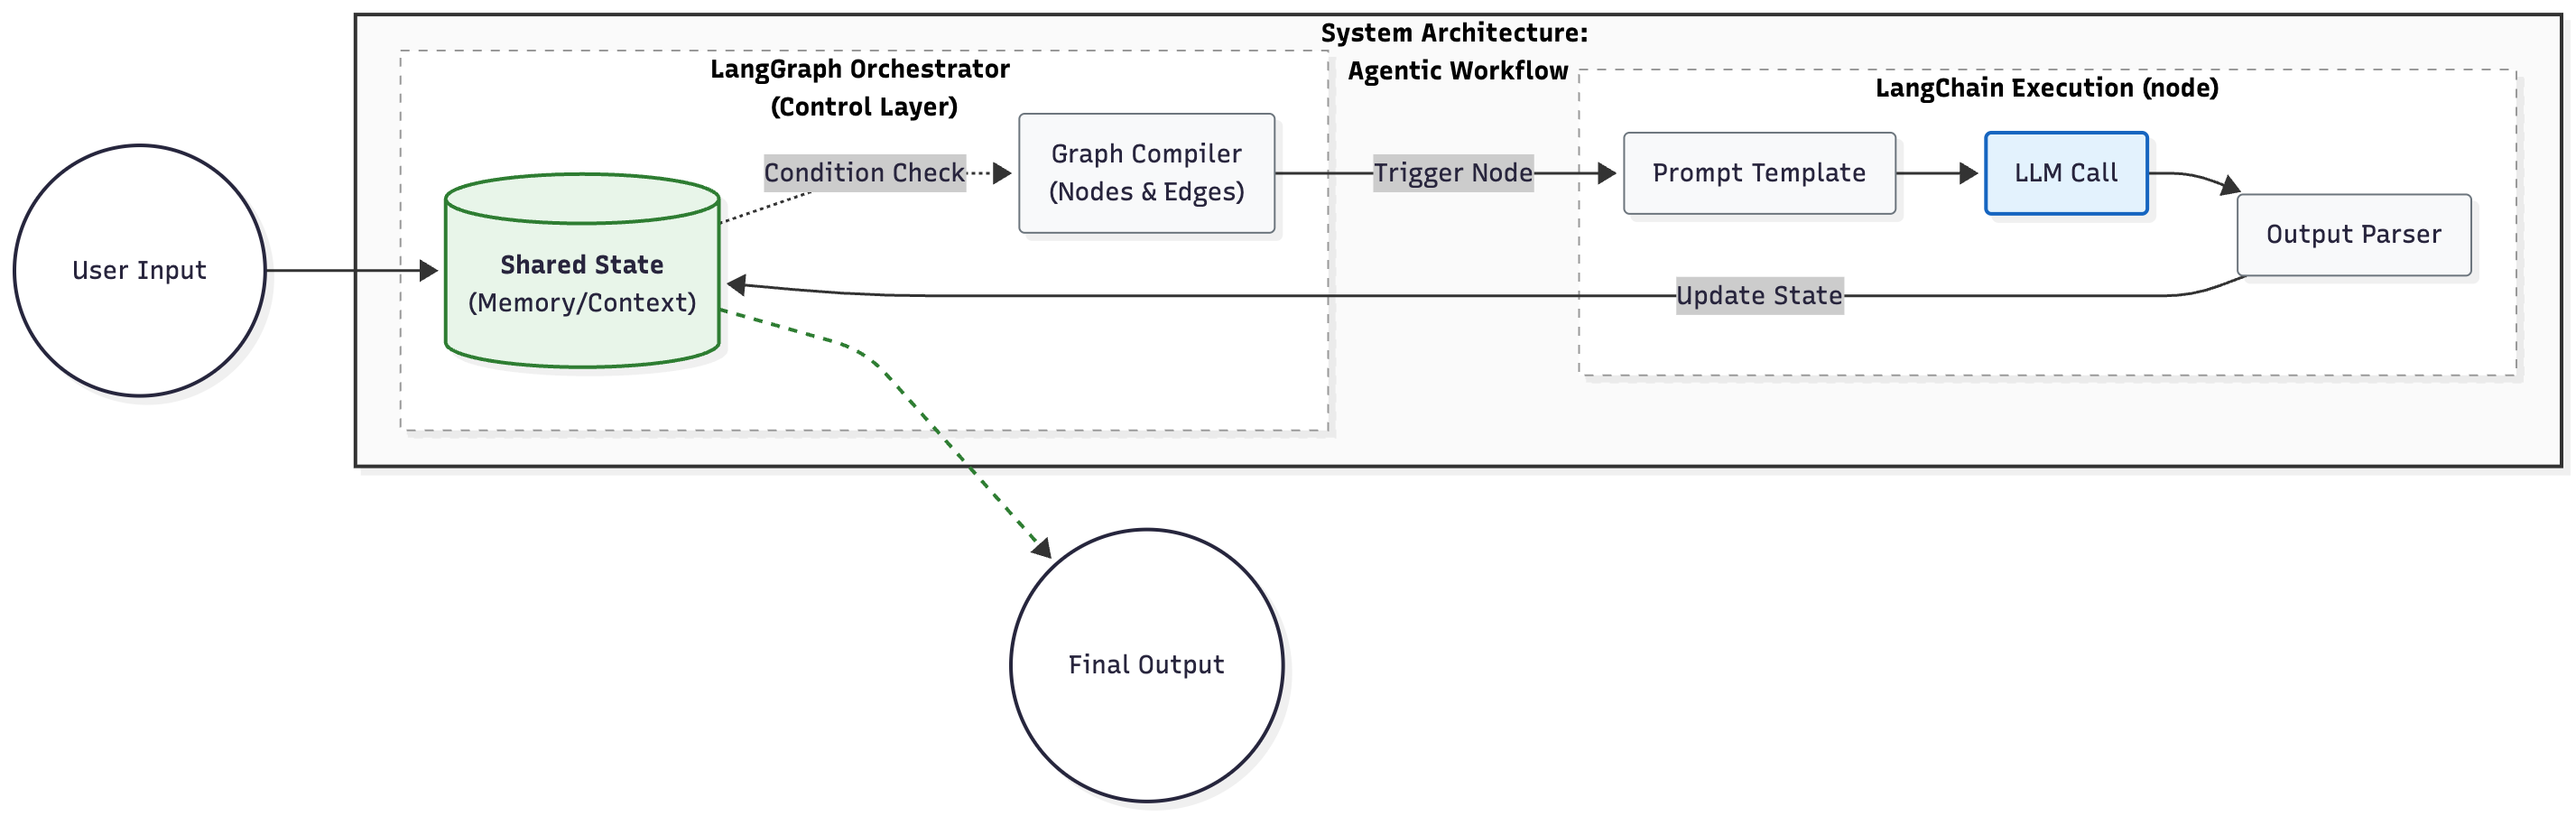
\includegraphics[width=0.88\textwidth]{figures/fig_langchain_integration.png}
\caption{LangChain and LangGraph integration architecture showing component composition and stateful workflow management.}
\label{fig:langchain}
\end{figure}

LangGraph represents workflows as directed graphs where nodes perform computational operations and edges define state transitions. The state is maintained through a typed dictionary that flows through the workflow:

\begin{equation}
\mathcal{S} = \{g, d, \delta, H, r, p, \theta, \sigma, \tau, \kappa, \alpha, \phi, M\}
\label{eq:state}
\end{equation}

where $g$ is grade level, $d$ is difficulty, $\delta$ is disability type, $H$ is student history, $r$ is student response, $p$ is the generated problem, $\theta$ is thought analysis, $\sigma$ is teaching strategies, $\tau$ is tutor session, $\kappa$ is consistency report, $\alpha$ is adaptive plan, $\phi$ is disability analysis, and $M$ is metadata.

\subsection{Prompt Engineering for Educational AI}

Effective prompt engineering is critical for generating authentic disability-specific simulations. Our approach follows five principles:

\textbf{Contextual Richness:} Each prompt embeds comprehensive disability characterizations. For disability $\delta$, we construct a knowledge tuple:

\begin{equation}
K_\delta = (D_\delta, C_\delta, I_\delta)
\label{eq:knowledge}
\end{equation}

where $D_\delta$ is the clinical description, $C_\delta = \{c_1, c_2, \ldots, c_n\}$ is the set of behavioral characteristics, and $I_\delta$ is the domain-specific impact statement.

\textbf{Temperature Calibration:} Different workflow stages require different creativity-consistency balances:

\begin{equation}
T(\text{task}) = \begin{cases}
0.5 & \text{problem\_generation} \\
1.0 & \text{student\_simulation} \\
0.3 & \text{cognitive\_analysis} \\
0.4 & \text{strategy\_generation} \\
0.7 & \text{tutor\_session} \\
0.2 & \text{validation}
\end{cases}
\label{eq:temperature}
\end{equation}

Tables~\ref{tab:prompt-engineering} and~\ref{tab:temperature} summarize the prompt engineering pipeline structure and temperature calibration.

\begin{table}[H]
\centering
\caption{Prompt Engineering Pipeline Structure}
\label{tab:prompt-engineering}
\footnotesize
\begin{tabular}{p{2cm}p{6cm}}
\toprule
\textbf{Component} & \textbf{Description} \\
\midrule
\textbf{Disability Profile} $P_\delta$ & 
$D_\delta$: Clinical description; $C_\delta$: Behavioral characteristics; $I_\delta$: Domain-specific impact \\
\addlinespace
\textbf{Prompt Construction} & 
System template; User context (problem, grade, difficulty); JSON schema \\
\addlinespace
\textbf{LLM Invocation} & 
GPT-4o-mini (128K context, JSON mode); Temperature $T$ (see Table~\ref{tab:temperature}); SHA256 cache \\
\bottomrule
\end{tabular}
\end{table}

\begin{table}[H]
\centering
\caption{Temperature Calibration by Task Type}
\label{tab:temperature}
\begin{tabular}{lcc}
\toprule
\textbf{Task Type} & \textbf{Temperature} & \textbf{Rationale} \\
\midrule
Problem Generation & 0.5 & Balanced creativity and consistency \\
Student Simulation & 1.0 & High variability for diverse error patterns \\
Cognitive Analysis & 0.3 & Consistent, deterministic reasoning \\
Strategy Generation & 0.4 & Semi-structured instructional content \\
Tutor Session & 0.7 & Natural, conversational dialogue \\
Consistency Validation & 0.2 & Deterministic validation checks \\
\bottomrule
\end{tabular}
\end{table}

\subsection{Cognitive Foundations of Learning Disabilities}

Our disability modeling is grounded in cognitive science research documenting how specific learning disabilities manifest in mathematical cognition:

\textbf{Dyslexia} affects reading and symbol processing, leading to digit reversals (6$\leftrightarrow$9, 3$\leftrightarrow$8), number transpositions (63$\rightarrow$36), and confusion with similar-looking symbols.

\textbf{Dyscalculia} directly impacts number sense, resulting in operation confusion, place value misunderstandings, and difficulty with mental math.

\textbf{ADHD} influences attention and executive function, manifesting as skipped steps, rushed calculations, and inconsistent performance.

\textbf{Dysgraphia} affects written expression, leading to miscopied numbers and disorganized calculations.

These profiles inform the parameterized prompts used in student simulation, ensuring generated responses reflect documented cognitive patterns rather than generic errors.

%-------------------------------------------------------------------------
\section{Method}\label{sec:method}

Our system architecture embodies three principles: modularity through workflow decomposition, quality through validation frameworks, and personalization through adaptive algorithms. Figure~\ref{fig:architecture} presents the complete system architecture.

\begin{figure}[H]
\centering
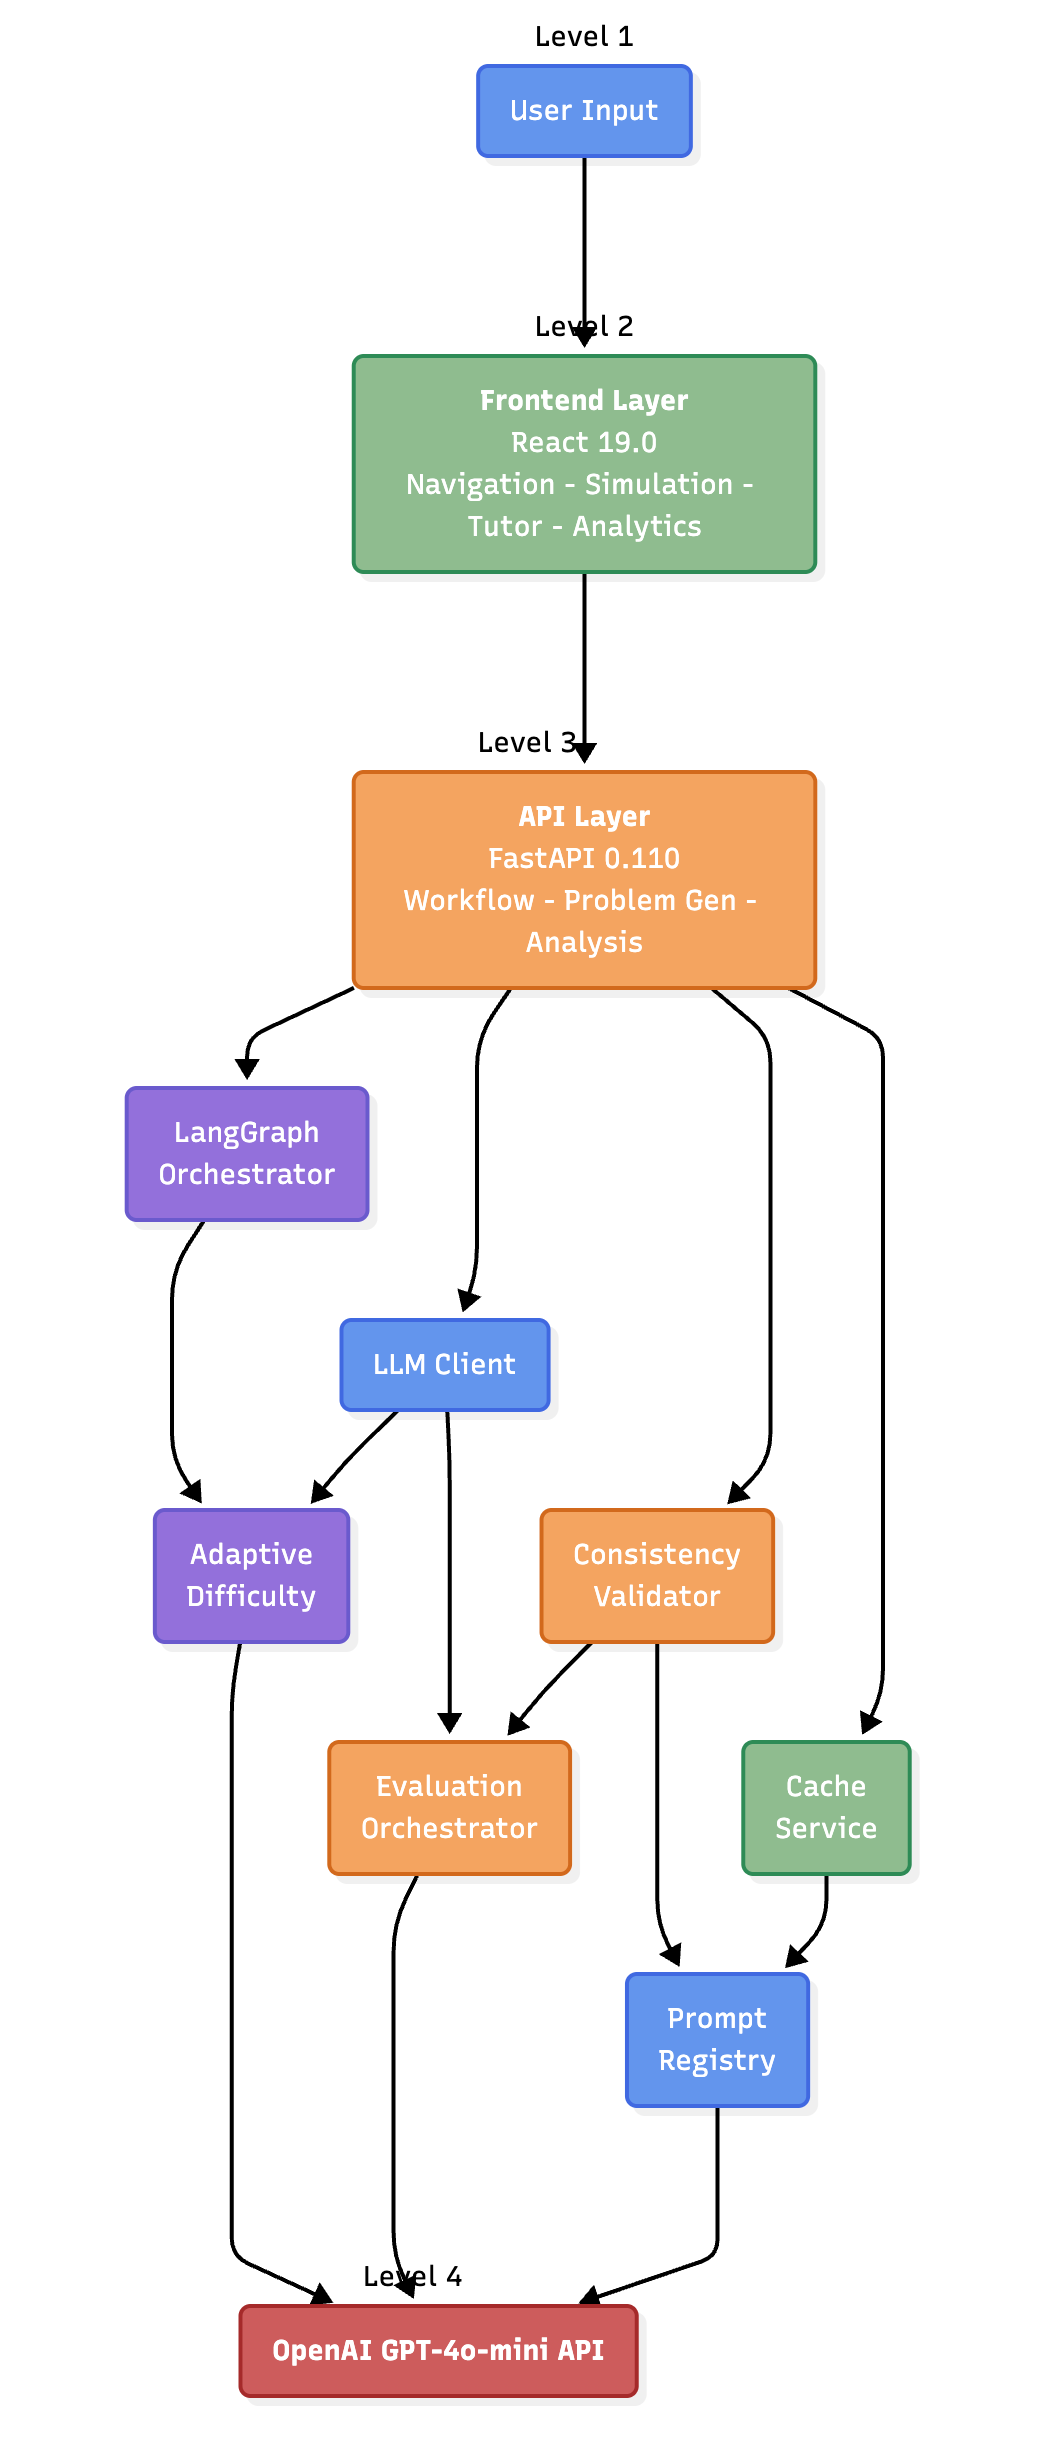
\includegraphics[width=0.42\textwidth]{figures/fig_system_architecture.png}
\caption{Four-layer system architecture: Frontend (React), API (FastAPI), Services, and External API (OpenAI).}
\label{fig:architecture}
\end{figure}

\subsection{LangGraph Workflow Architecture}

The primary workflow consists of eight interconnected nodes implementing specific educational assessment functions. Figure~\ref{fig:workflow} illustrates the complete workflow graph.

\begin{figure}[H]
\centering
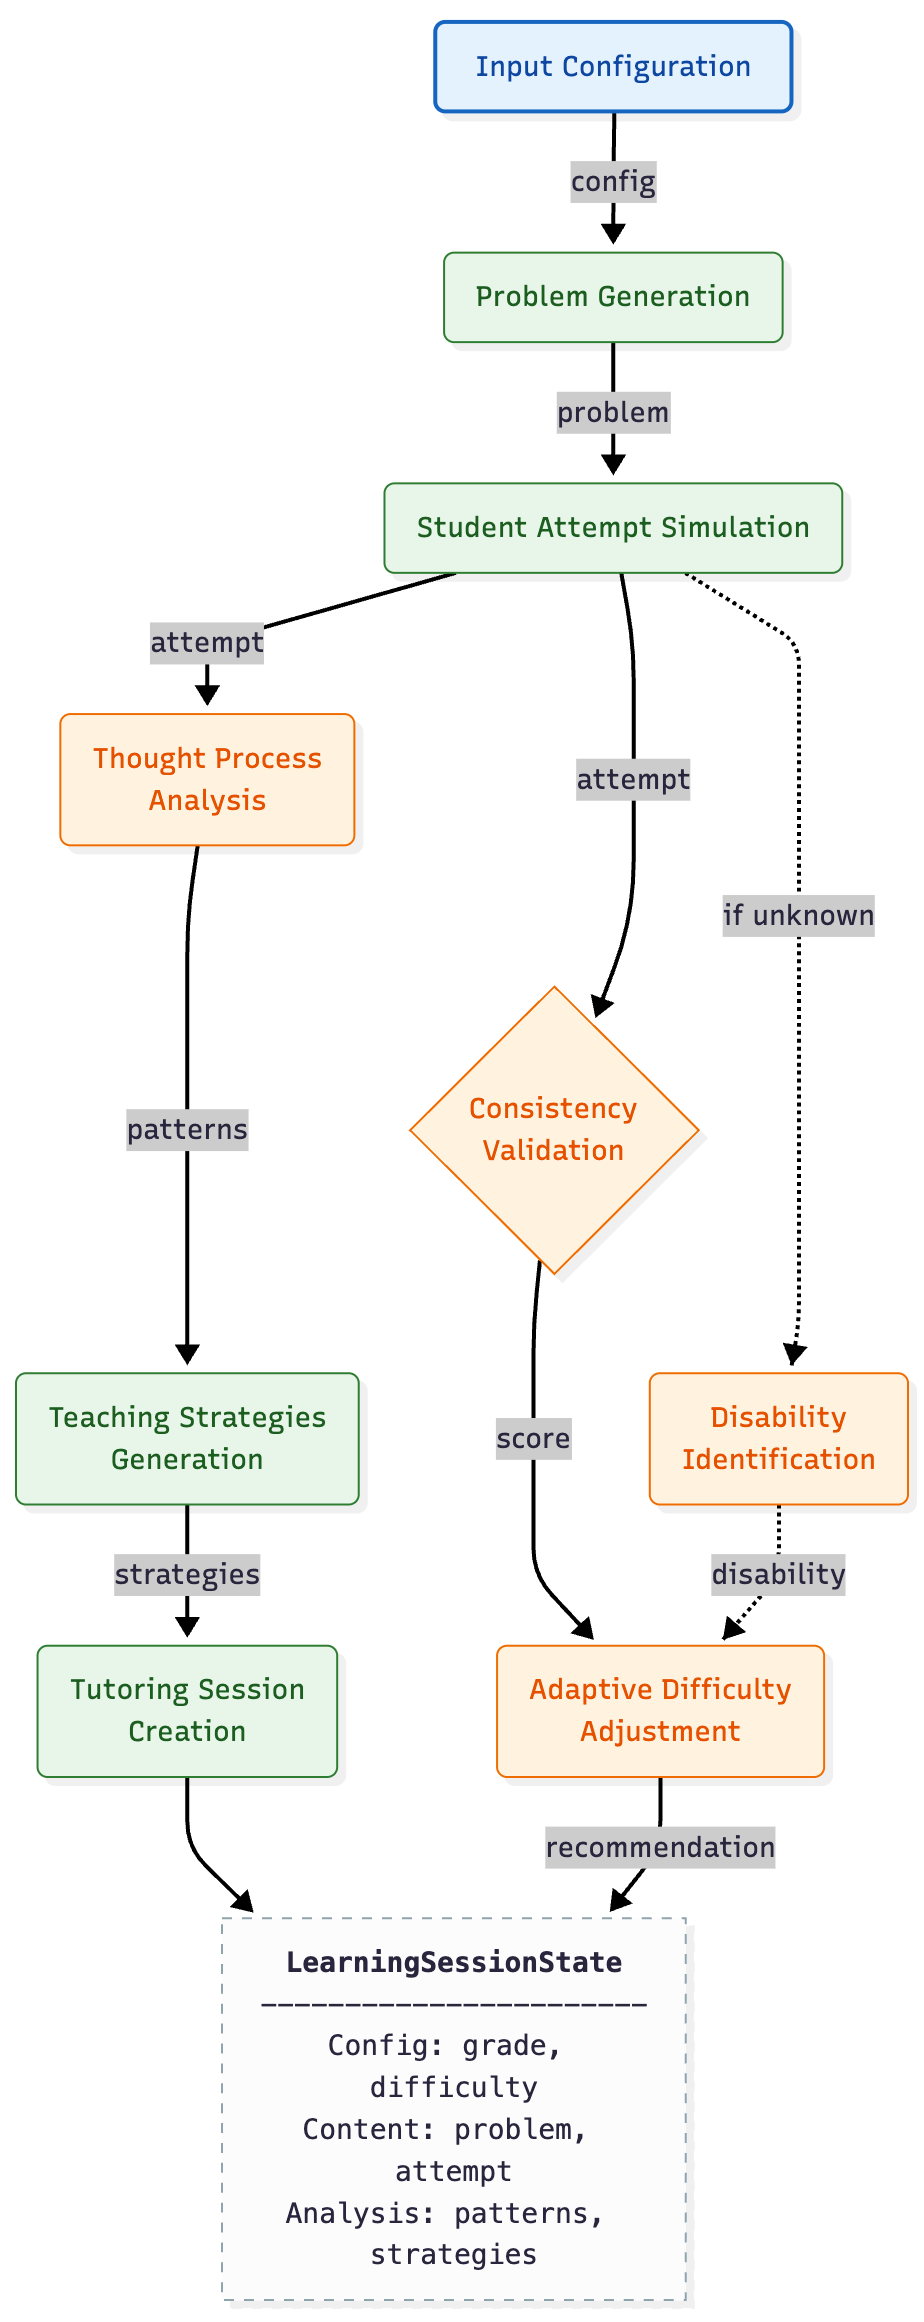
\includegraphics[width=0.48\textwidth]{figures/fig_langgraph_workflow.png}
\caption{LangGraph workflow showing problem generation, student simulation, analysis, validation, and tutoring session creation.}
\label{fig:workflow}
\end{figure}

Each node is implemented as an async method in the LangGraphOrchestrator class:

\begin{enumerate}
    \item \textbf{Problem Generation Node} ($n_1$, $T=0.5$): Creates age-appropriate mathematics word problems using structured prompts incorporating grade level and difficulty constraints.
    
    \item \textbf{Student Attempt Simulation Node} ($n_2$, $T=1.0$): Generates realistic student responses using disability-specific prompts with high temperature for diverse error patterns.
    
    \item \textbf{Thought Process Analysis Node} ($n_3$, $T=0.3$): Performs deep cognitive analysis identifying error types and disability-specific manifestations.
    
    \item \textbf{Teaching Strategies Generation Node} ($n_4$, $T=0.4$): Develops evidence-based instructional approaches with primary strategies, alternative approaches, and accommodations.
    
    \item \textbf{Tutoring Session Creation Node} ($n_5$, $T=0.7$): Synthesizes analyses into interactive tutor-student dialogues with 10--12 exchanges.
    
    \item \textbf{Consistency Validation Node} ($n_6$, $T=0.2$): Validates response authenticity through multi-dimensional analysis.
    
    \item \textbf{Adaptive Difficulty Adjustment Node} ($n_7$, $T=0.3$): Analyzes longitudinal performance data for difficulty recommendations.
    
    \item \textbf{Disability Identification Node} ($n_8$, $T=0.2$): Analyzes student work patterns to identify potential learning disabilities.
\end{enumerate}

\subsection{Consistency Validation Framework}

The Consistency Validation Node computes an overall consistency score as a weighted average of five orthogonal metrics.

The overall consistency score is computed as:

\begin{equation}
\kappa(r, \delta) = \sum_{i=1}^{5} w_i \cdot v_i(r, \delta)
\label{eq:consistency}
\end{equation}

where weights $w = [0.25, 0.25, 0.15, 0.20, 0.15]$ prioritize disability authenticity and solution coherence.

\textbf{Step-Answer Consistency} ($v_1$): Verifies that the final answer appears in the step-by-step work:

\begin{equation}
v_1(r) = \begin{cases}
1.0 & \text{if } a_{\text{final}} \in \text{extract}(S) \\
0.3 & \text{otherwise}
\end{cases}
\label{eq:step_answer}
\end{equation}

\textbf{Disability-Specific Behavior} ($v_2$): Analyzes the frequency of expected behaviors $B_\delta^+$ and penalizes unexpected behaviors $B_\delta^-$:

\begin{equation}
v_2(r, \delta) = \min\left(1.0, \frac{|B_\delta^+ \cap B(r)|}{0.3 \cdot |B_\delta^+|}\right) - 0.5 \cdot \frac{|B_\delta^- \cap B(r)|}{|B_\delta^-|}
\label{eq:behavior}
\end{equation}

\textbf{Mathematical Reasoning} ($v_3$): Evaluates logical progression:

\begin{equation}
v_3(r) = \frac{1}{3}\left(\mathbb{1}_{\text{ops}} + \mathbb{1}_{\text{prog}} + \mathbb{1}_{\text{reasonable}}\right)
\label{eq:math_reasoning}
\end{equation}

\textbf{Error Pattern Consistency} ($v_4$): Validates that errors match expected patterns for disability $\delta$:

\begin{equation}
v_4(r, \delta) = \frac{|E_\delta \cap E(r)|}{|E_\delta|}
\label{eq:error_patterns}
\end{equation}

\textbf{Response Completeness} ($v_5$): Ensures all required fields contain meaningful content:

\begin{equation}
v_5(r) = \frac{1}{2}\left(\frac{|\text{present\_fields}|}{|\text{required\_fields}|} + \frac{\text{meaningful\_steps}}{\text{total\_steps}}\right)
\label{eq:completeness}
\end{equation}

\subsection{Adaptive Difficulty Algorithm}

The adaptive difficulty algorithm analyzes performance history to recommend appropriate difficulty adjustments. The algorithm operates on performance history $H = \{(r_i, \kappa_i, a_i)\}_{i=1}^{n}$. From the most recent $k=5$ sessions, we compute:

\begin{align}
\bar{\kappa} &= \frac{1}{k}\sum_{i=n-k+1}^{n} \kappa_i, \quad
\bar{a} = \frac{1}{k}\sum_{i=n-k+1}^{n} a_i, \quad
\kappa_{\max} = \max_{i \in [n-k+1, n]} \kappa_i
\end{align}

The trend coefficient $\beta$ measures performance trajectory:

\begin{equation}
\beta = \frac{\bar{\kappa}_{\text{late}} - \bar{\kappa}_{\text{early}}}{k/2}
\label{eq:trend}
\end{equation}

The difficulty adjustment decision follows:

\begin{equation}
\Delta\ell = \begin{cases}
+1 & \text{if } \bar{a} \geq 0.8 \land \bar{\kappa} \geq 0.75 \land \kappa_{\max} \geq 0.85 \\[0.3em]
-1 & \text{if } \bar{a} \leq 0.45 \lor \bar{\kappa} \leq 0.4 \lor (\beta < -0.1 \land \bar{\kappa} < 0.6) \\[0.3em]
0 & \text{otherwise}
\end{cases}
\label{eq:difficulty_decision}
\end{equation}

Algorithm~\ref{alg:adaptive} presents the pseudocode for the adaptive difficulty adjustment.

\begin{algorithm}[H]
\caption{Adaptive Difficulty Adjustment}
\label{alg:adaptive}
\begin{algorithmic}[1]
\Require Performance history $H = \{(r_i, \kappa_i, a_i)\}_{i=1}^{n}$, current difficulty $\ell$
\Ensure Difficulty adjustment $\Delta\ell \in \{-1, 0, +1\}$
\State Extract recent $k \gets 5$ sessions: $H_{\text{recent}} \gets H[n-k+1:n]$
\State Compute metrics:
\State \quad $\bar{\kappa} \gets \frac{1}{k}\sum_{i=1}^{k} \kappa_i$
\State \quad $\bar{a} \gets \frac{1}{k}\sum_{i=1}^{k} a_i$
\State \quad $\kappa_{\max} \gets \max\{\kappa_i : i \in [1, k]\}$
\State Compute trend: $\beta \gets \frac{\bar{\kappa}_{\text{late}} - \bar{\kappa}_{\text{early}}}{k/2}$
\If{$\bar{a} \geq 0.8 \land \bar{\kappa} \geq 0.75 \land \kappa_{\max} \geq 0.85$}
    \State $\Delta\ell \gets +1$ \Comment{Increase difficulty}
    \State \Return $\Delta\ell$
\ElsIf{$\bar{a} \leq 0.45 \lor \bar{\kappa} \leq 0.4 \lor (\beta < -0.1 \land \bar{\kappa} < 0.6)$}
    \State $\Delta\ell \gets -1$ \Comment{Decrease difficulty}
    \State \Return $\Delta\ell$
\Else
    \State $\Delta\ell \gets 0$ \Comment{Maintain current level}
    \State \Return $\Delta\ell$
\EndIf
\end{algorithmic}
\end{algorithm}

\subsection{Analytics Visualizations}

The system provides comprehensive analytics visualizations for tracking student performance over time. Figure~\ref{fig:analytics-performance} shows the temporal performance tracking, and Figure~\ref{fig:analytics-errors} shows the error pattern analysis.

\begin{figure}[H]
\centering
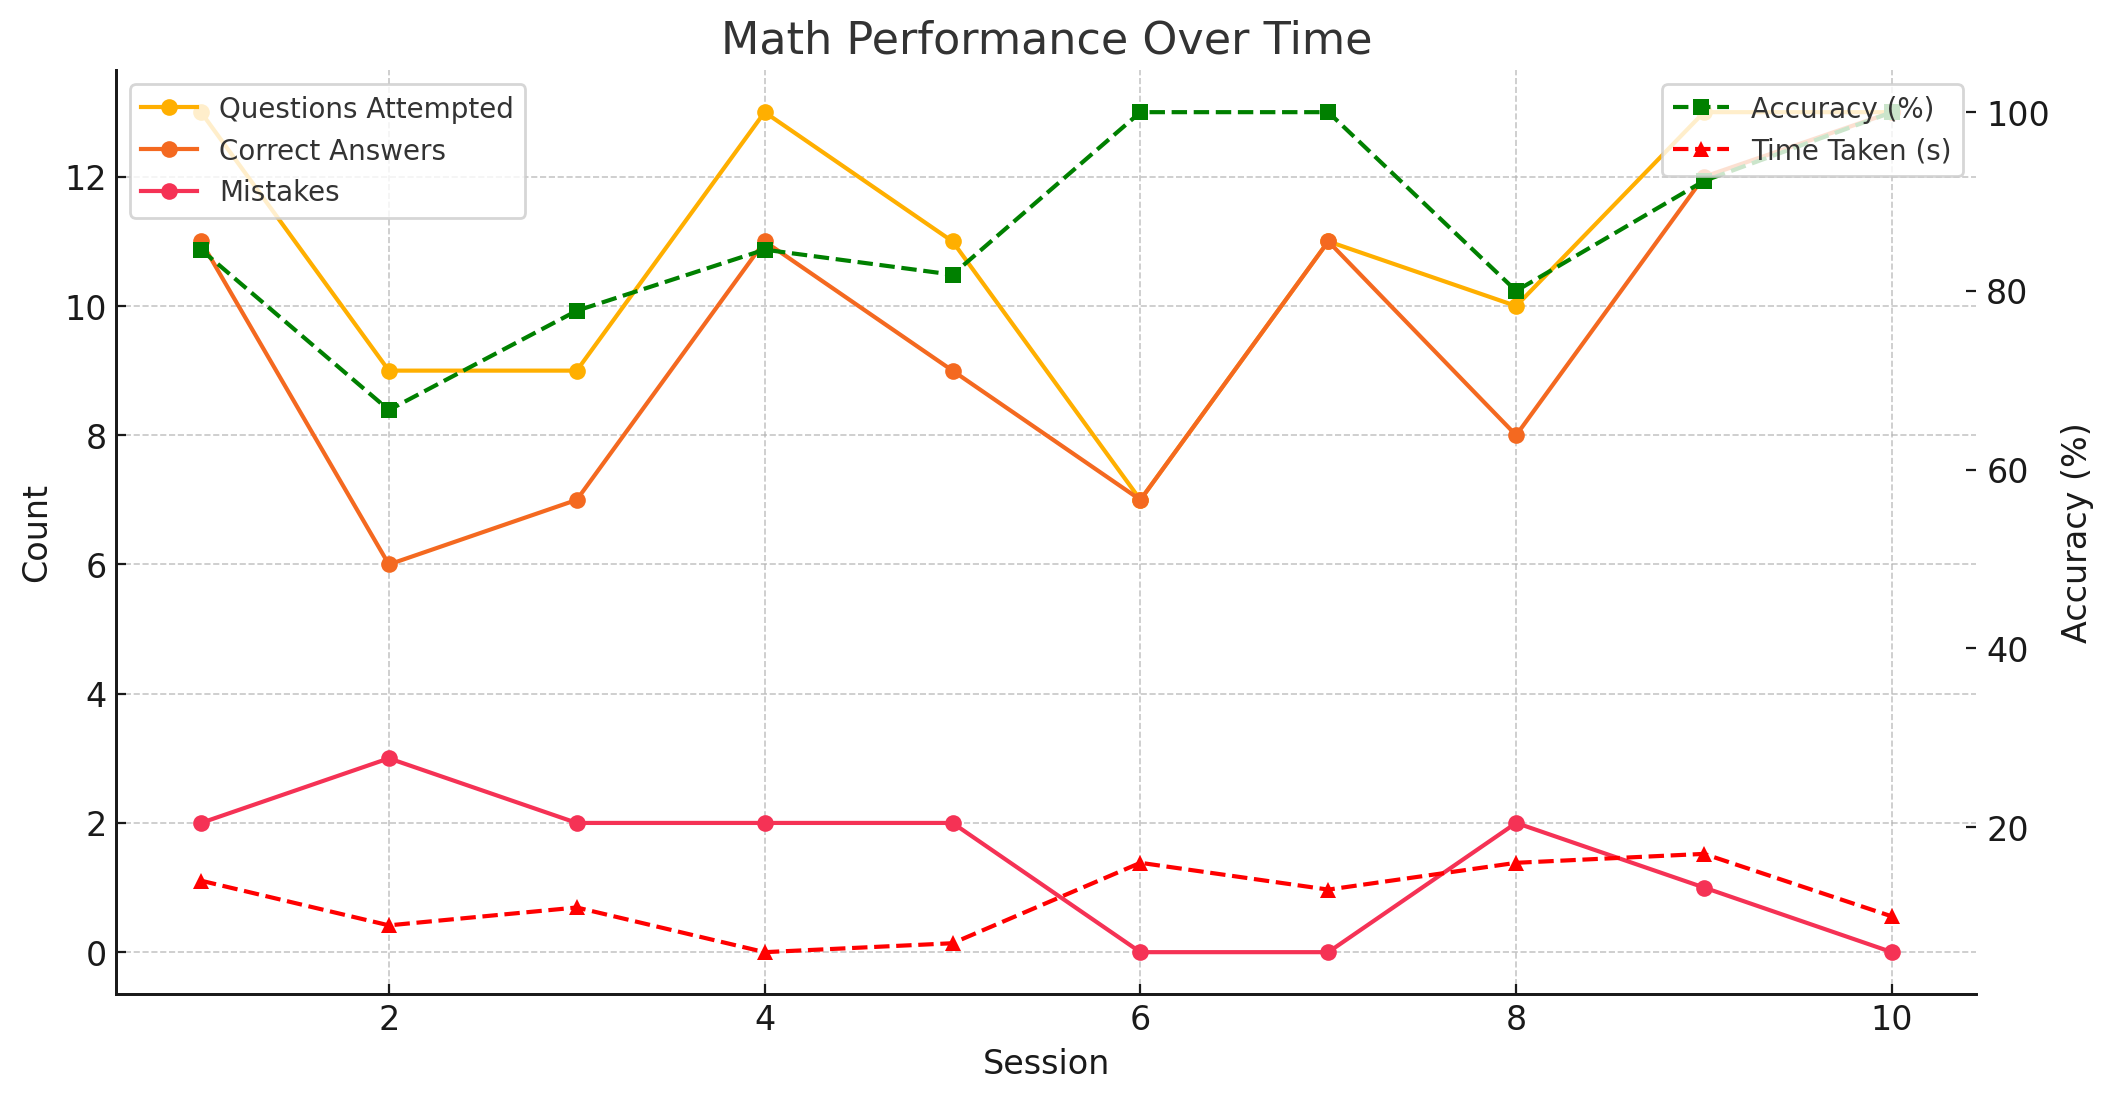
\includegraphics[width=0.78\textwidth]{figures/output-1.png}
\caption{Temporal performance tracking: questions, accuracy, and time across sessions.}
\label{fig:analytics-performance}
\end{figure}

\begin{figure}[H]
\centering
\begin{minipage}{0.44\textwidth}
\centering
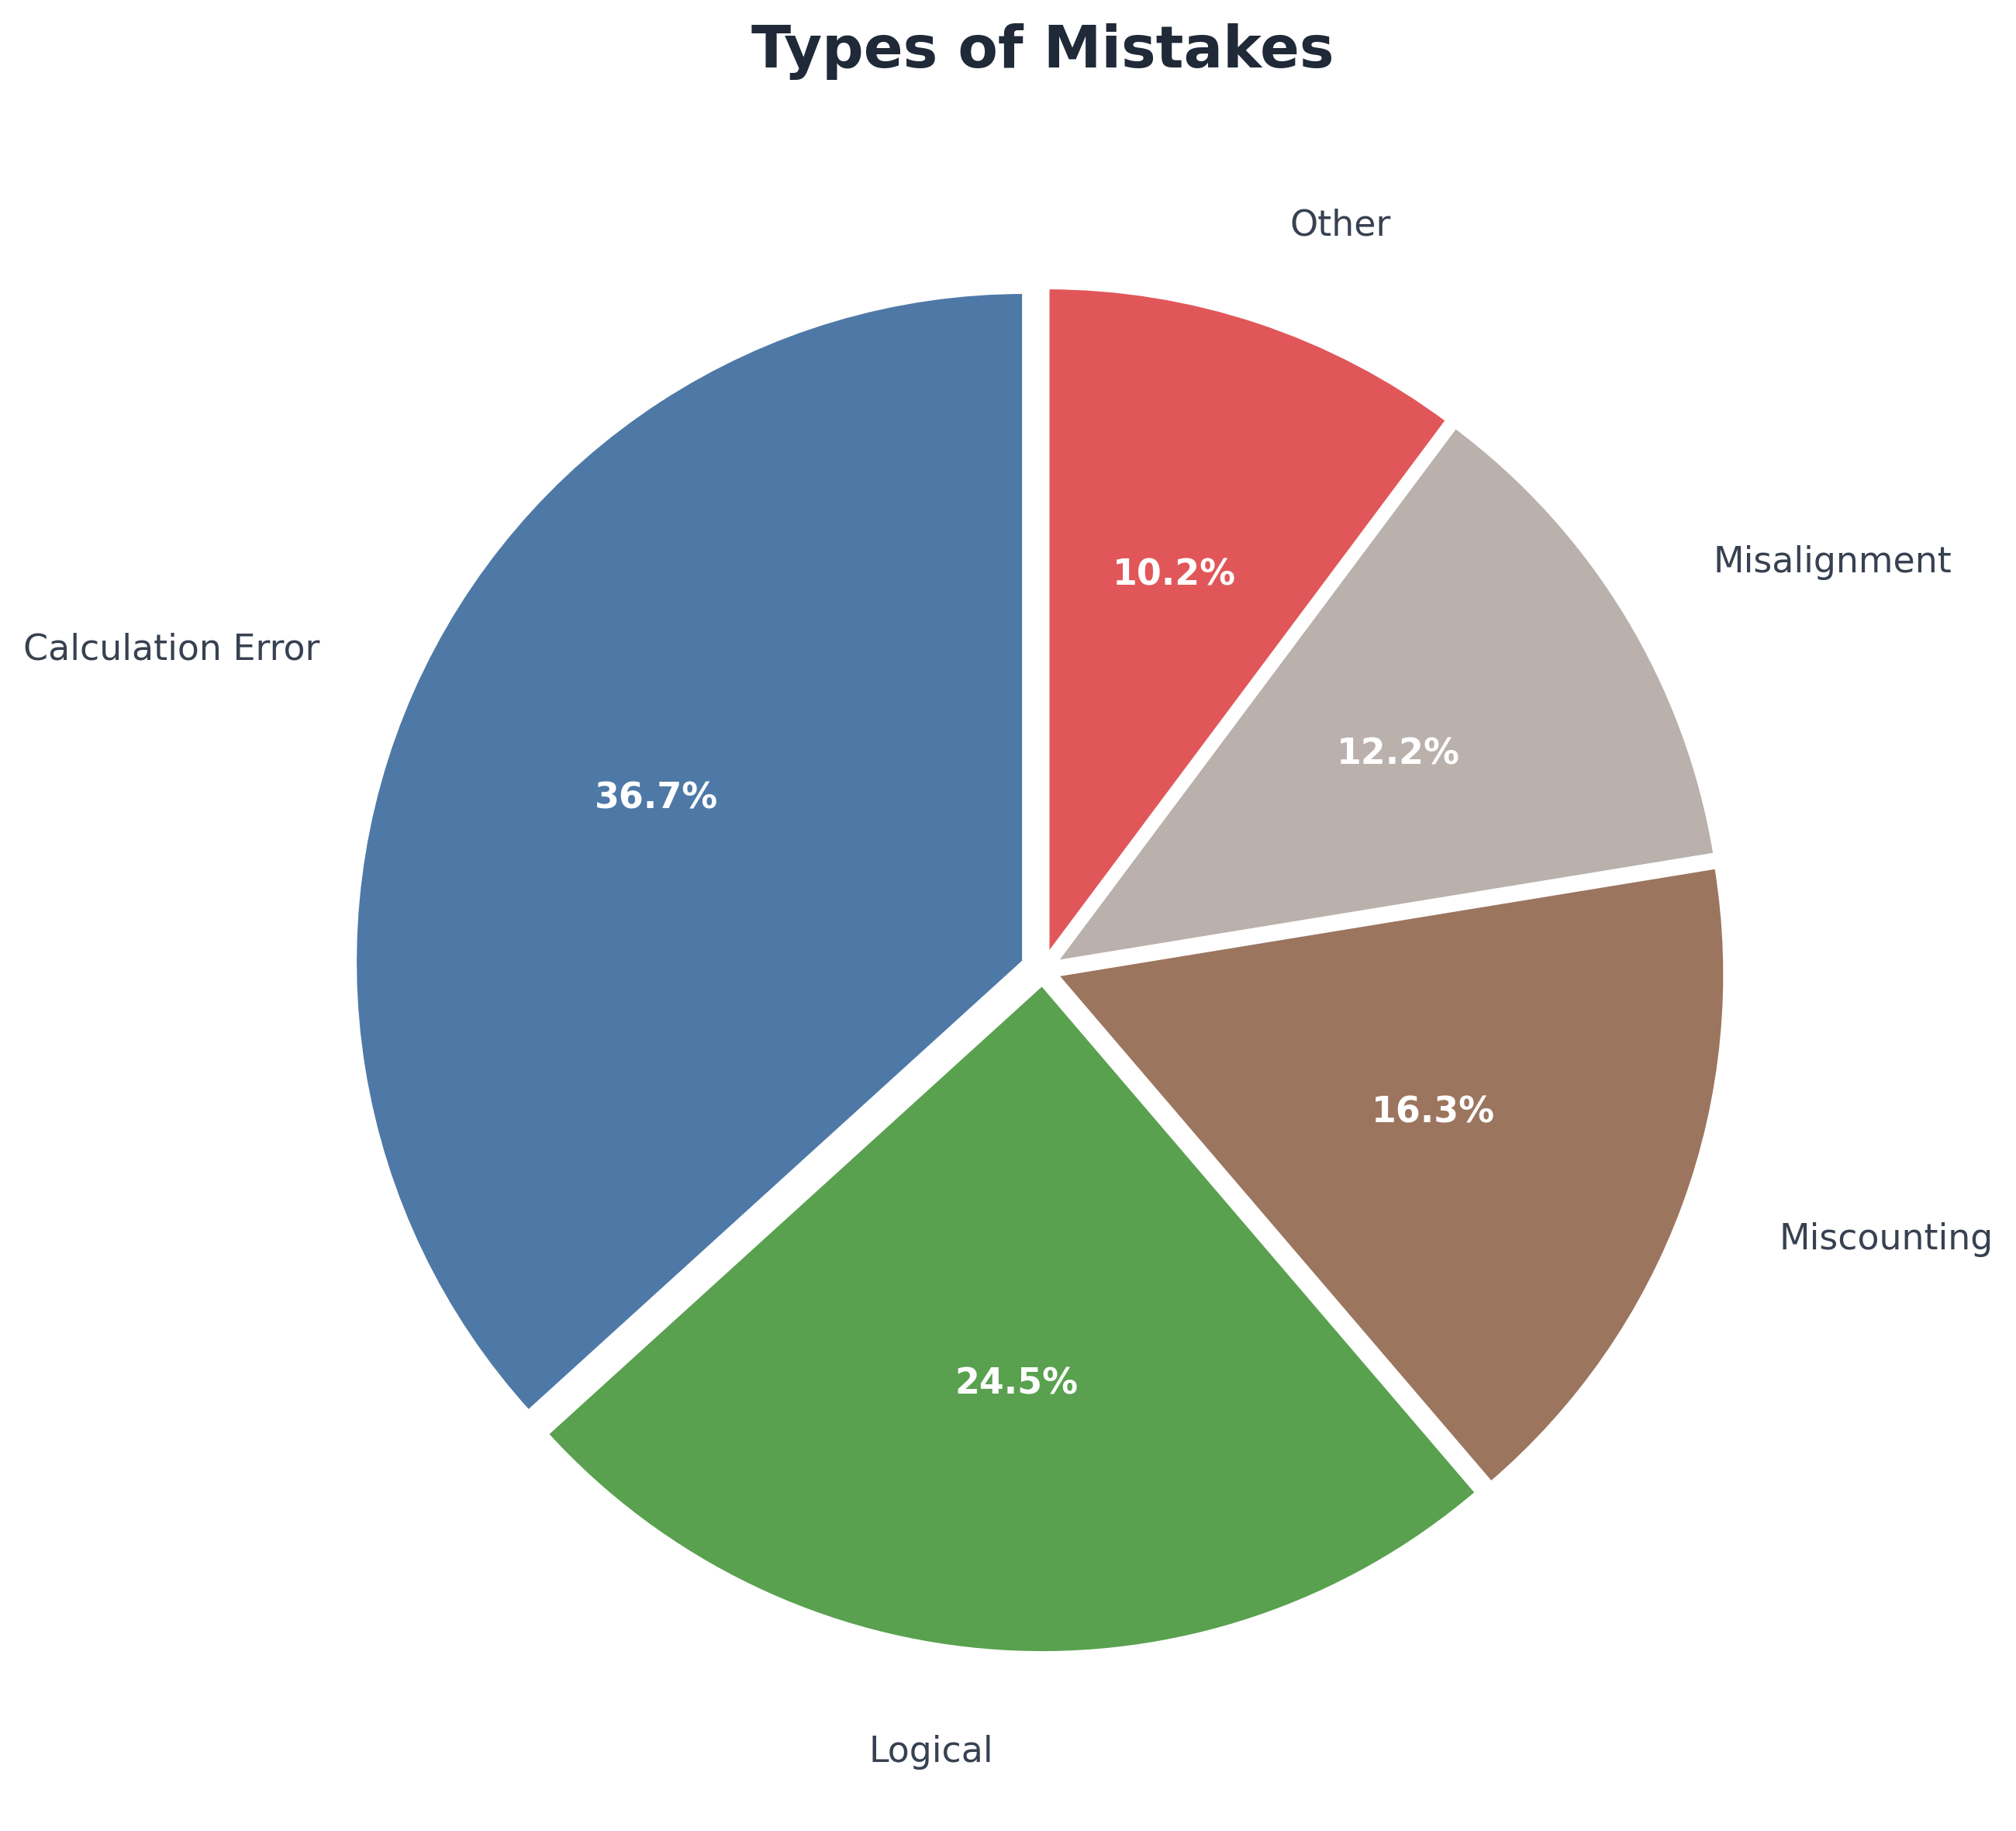
\includegraphics[width=\textwidth]{figures/output-2.png}
\end{minipage}
\hfill
\begin{minipage}{0.44\textwidth}
\centering
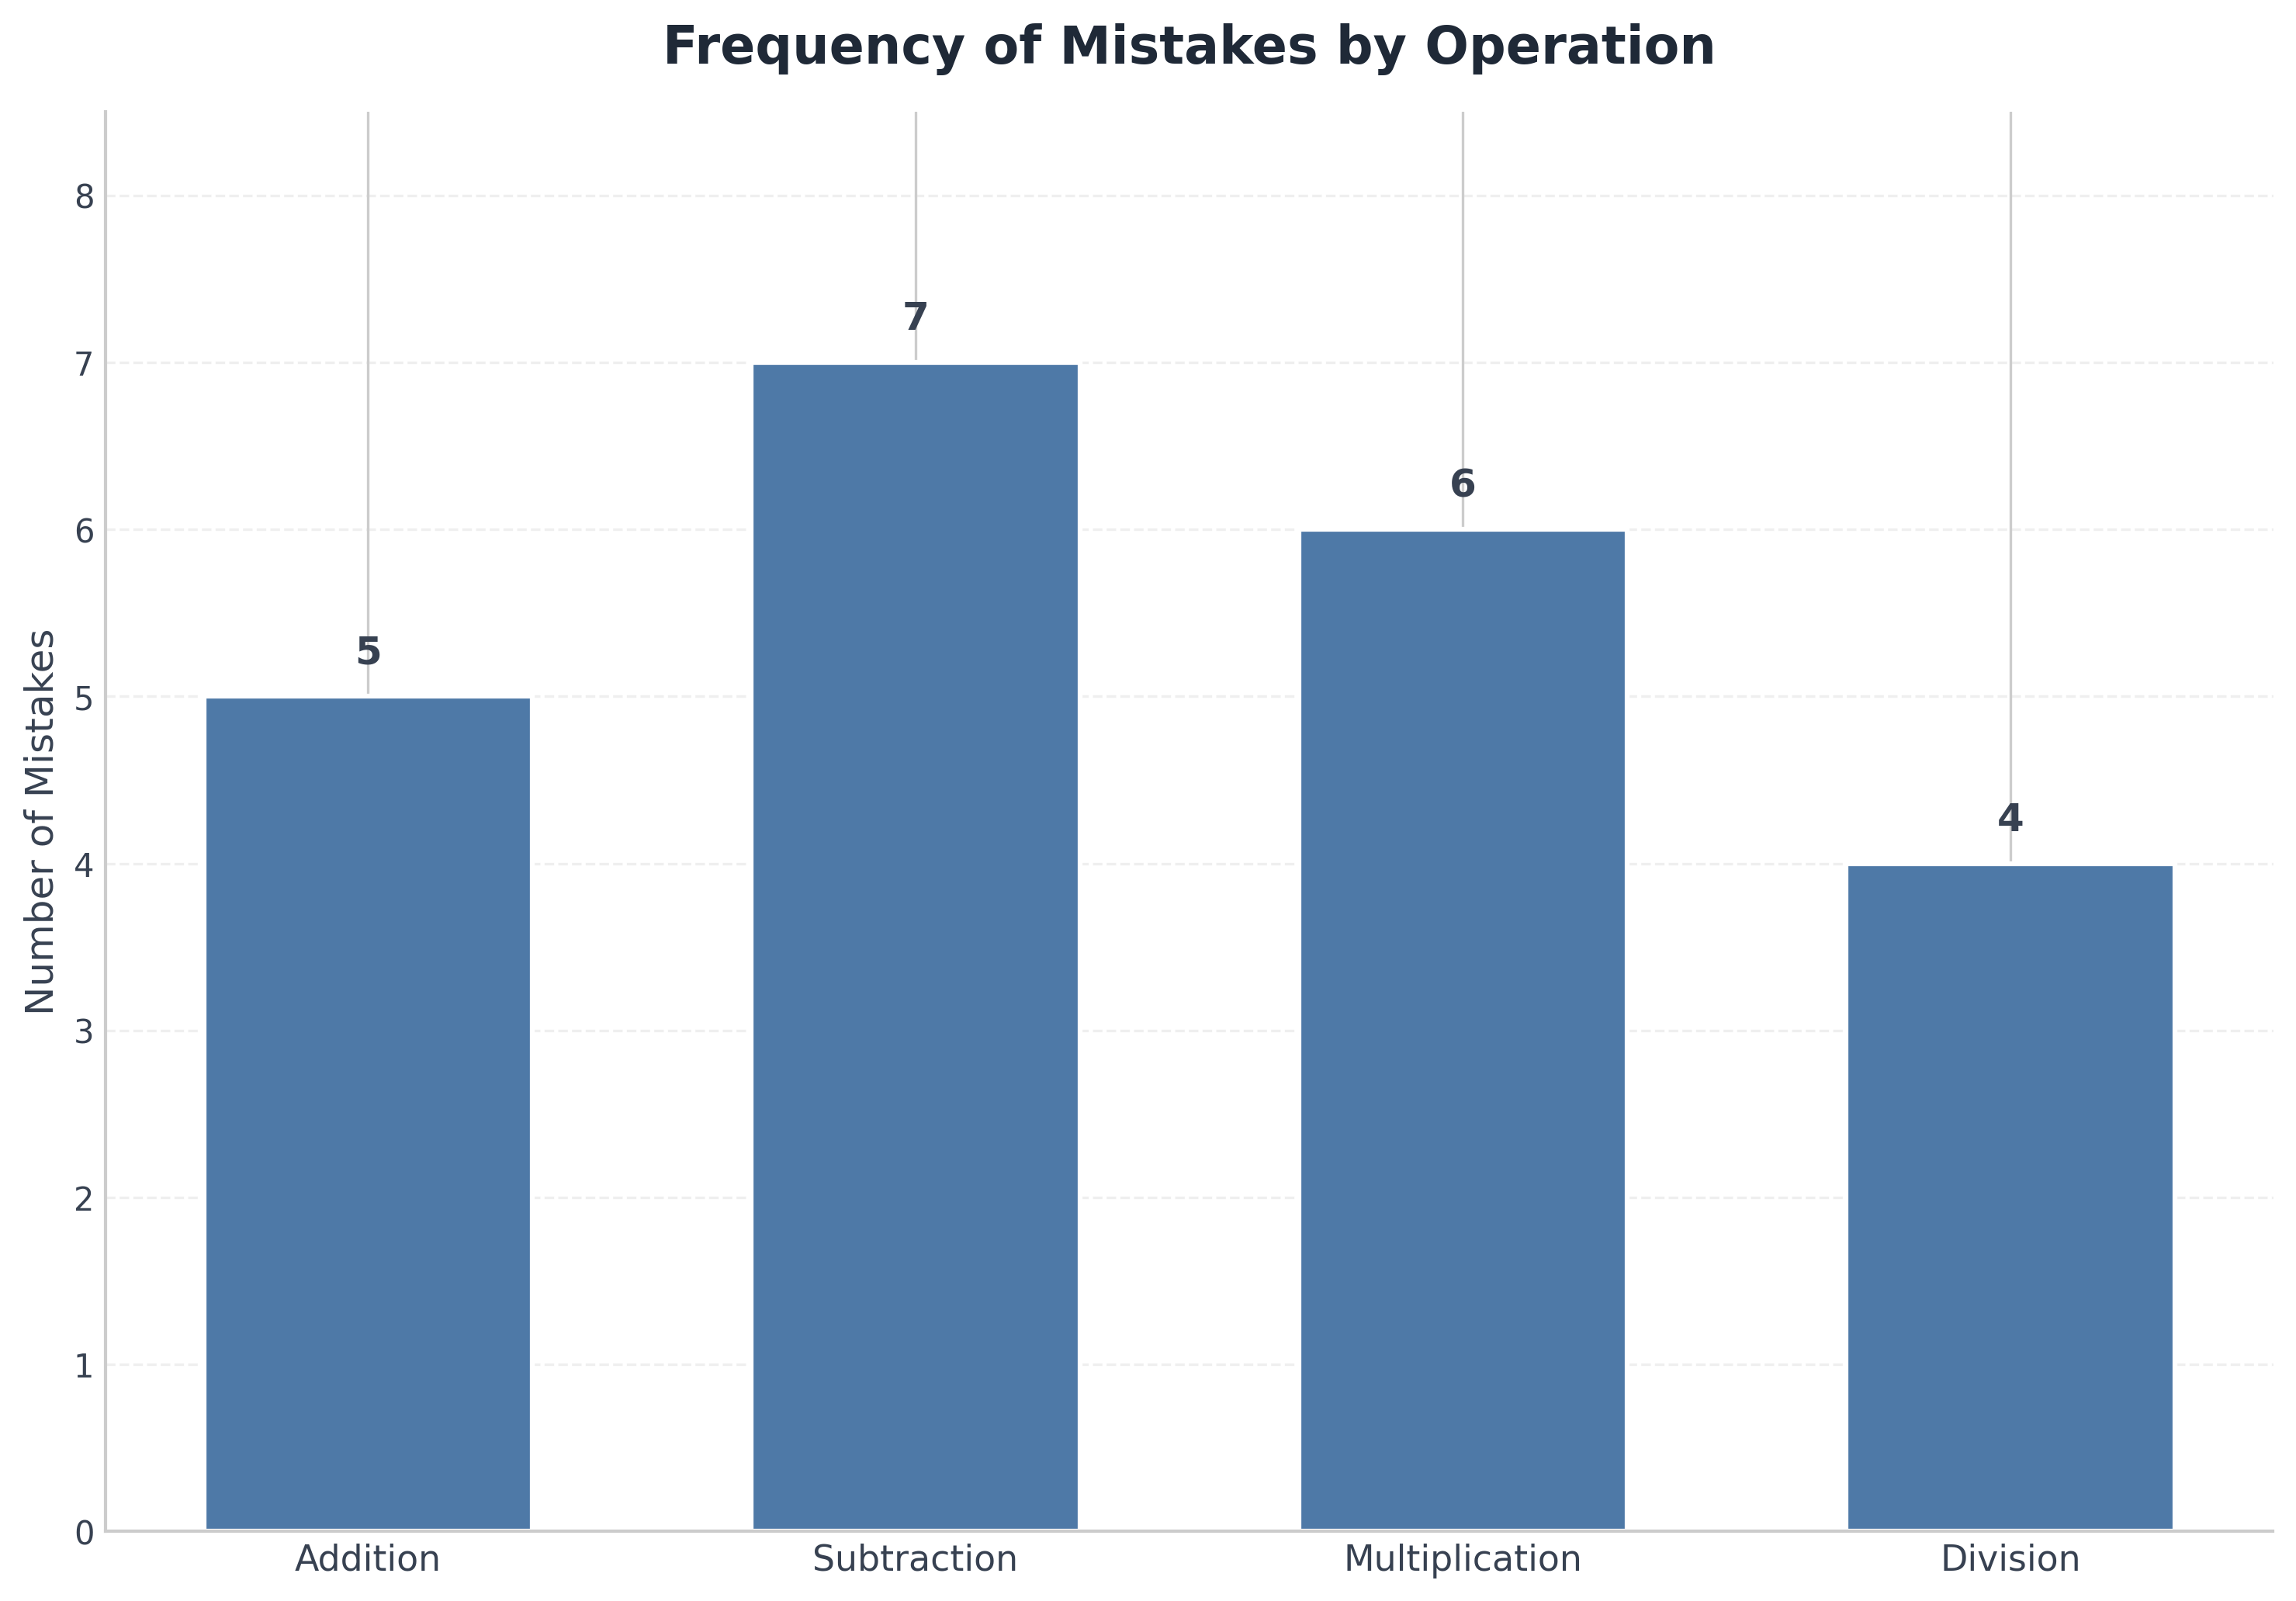
\includegraphics[width=\textwidth]{figures/output-3.png}
\end{minipage}
\caption{Error analysis: (Left) Mistake type distribution. (Right) Mistakes by operation.}
\label{fig:analytics-errors}
\end{figure}

\begin{figure}[H]
\centering
\begin{minipage}{0.44\textwidth}
\centering
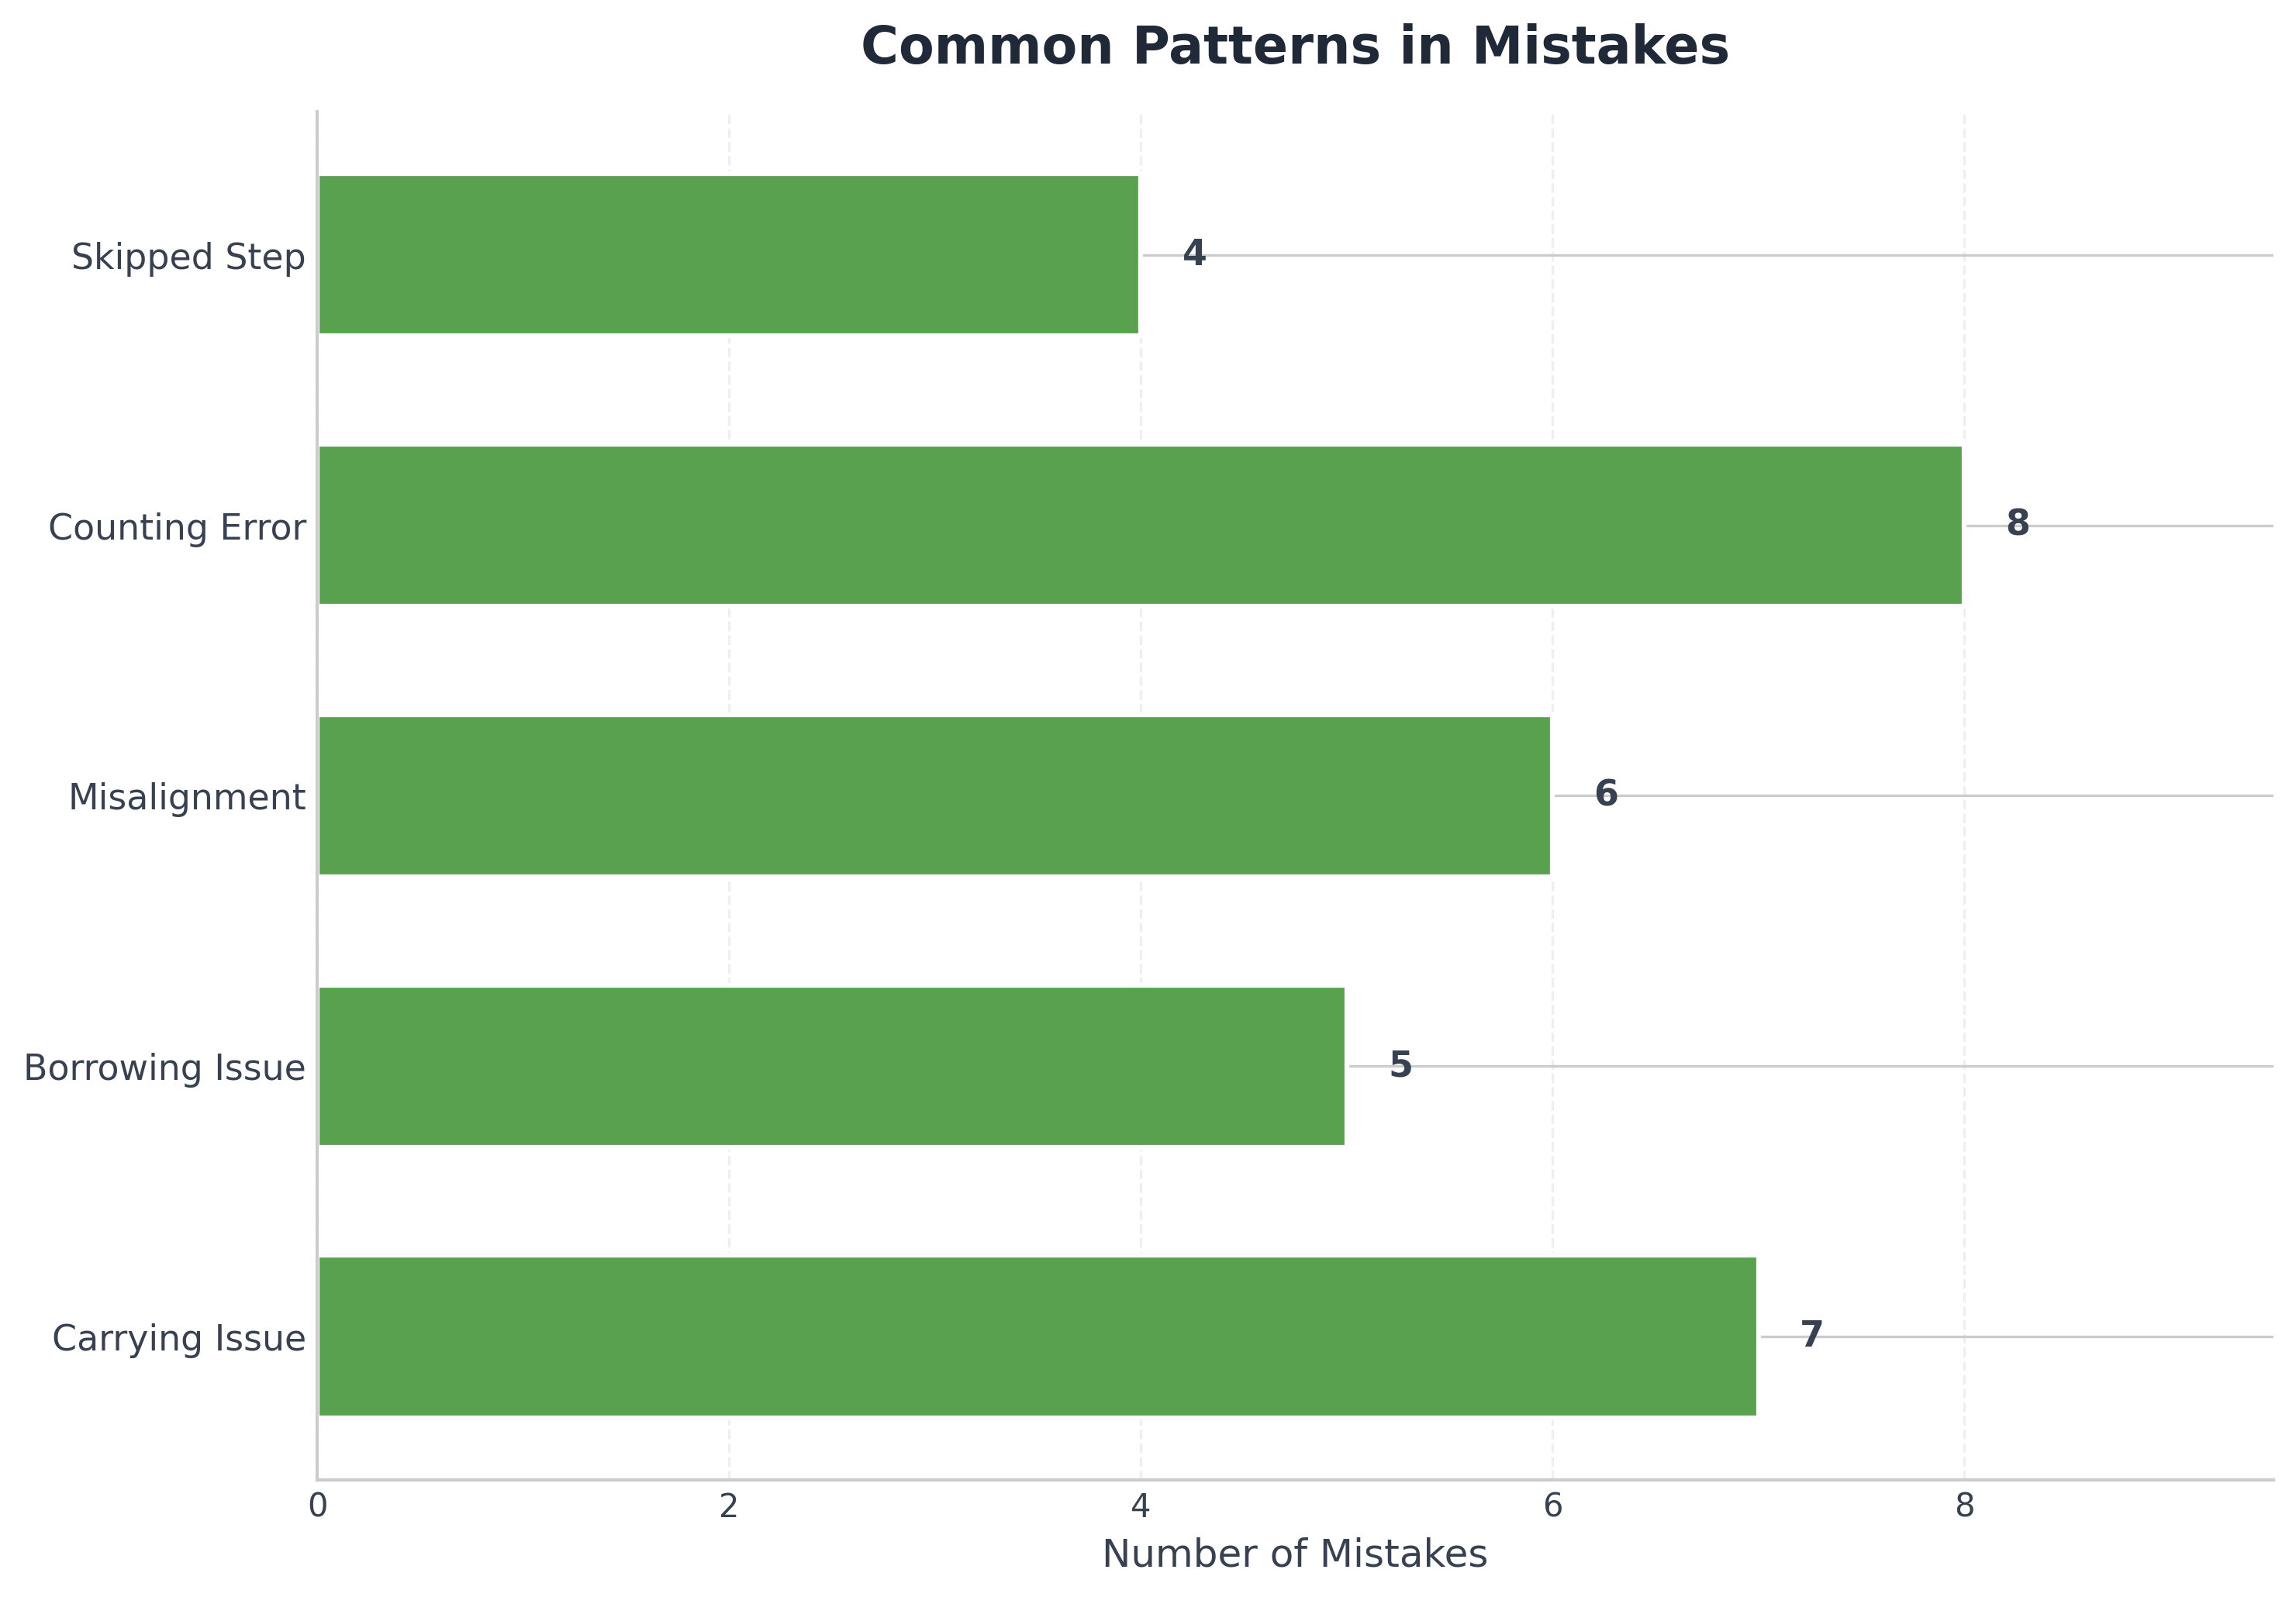
\includegraphics[width=\textwidth]{figures/output-4.png}
\end{minipage}
\hfill
\begin{minipage}{0.44\textwidth}
\centering
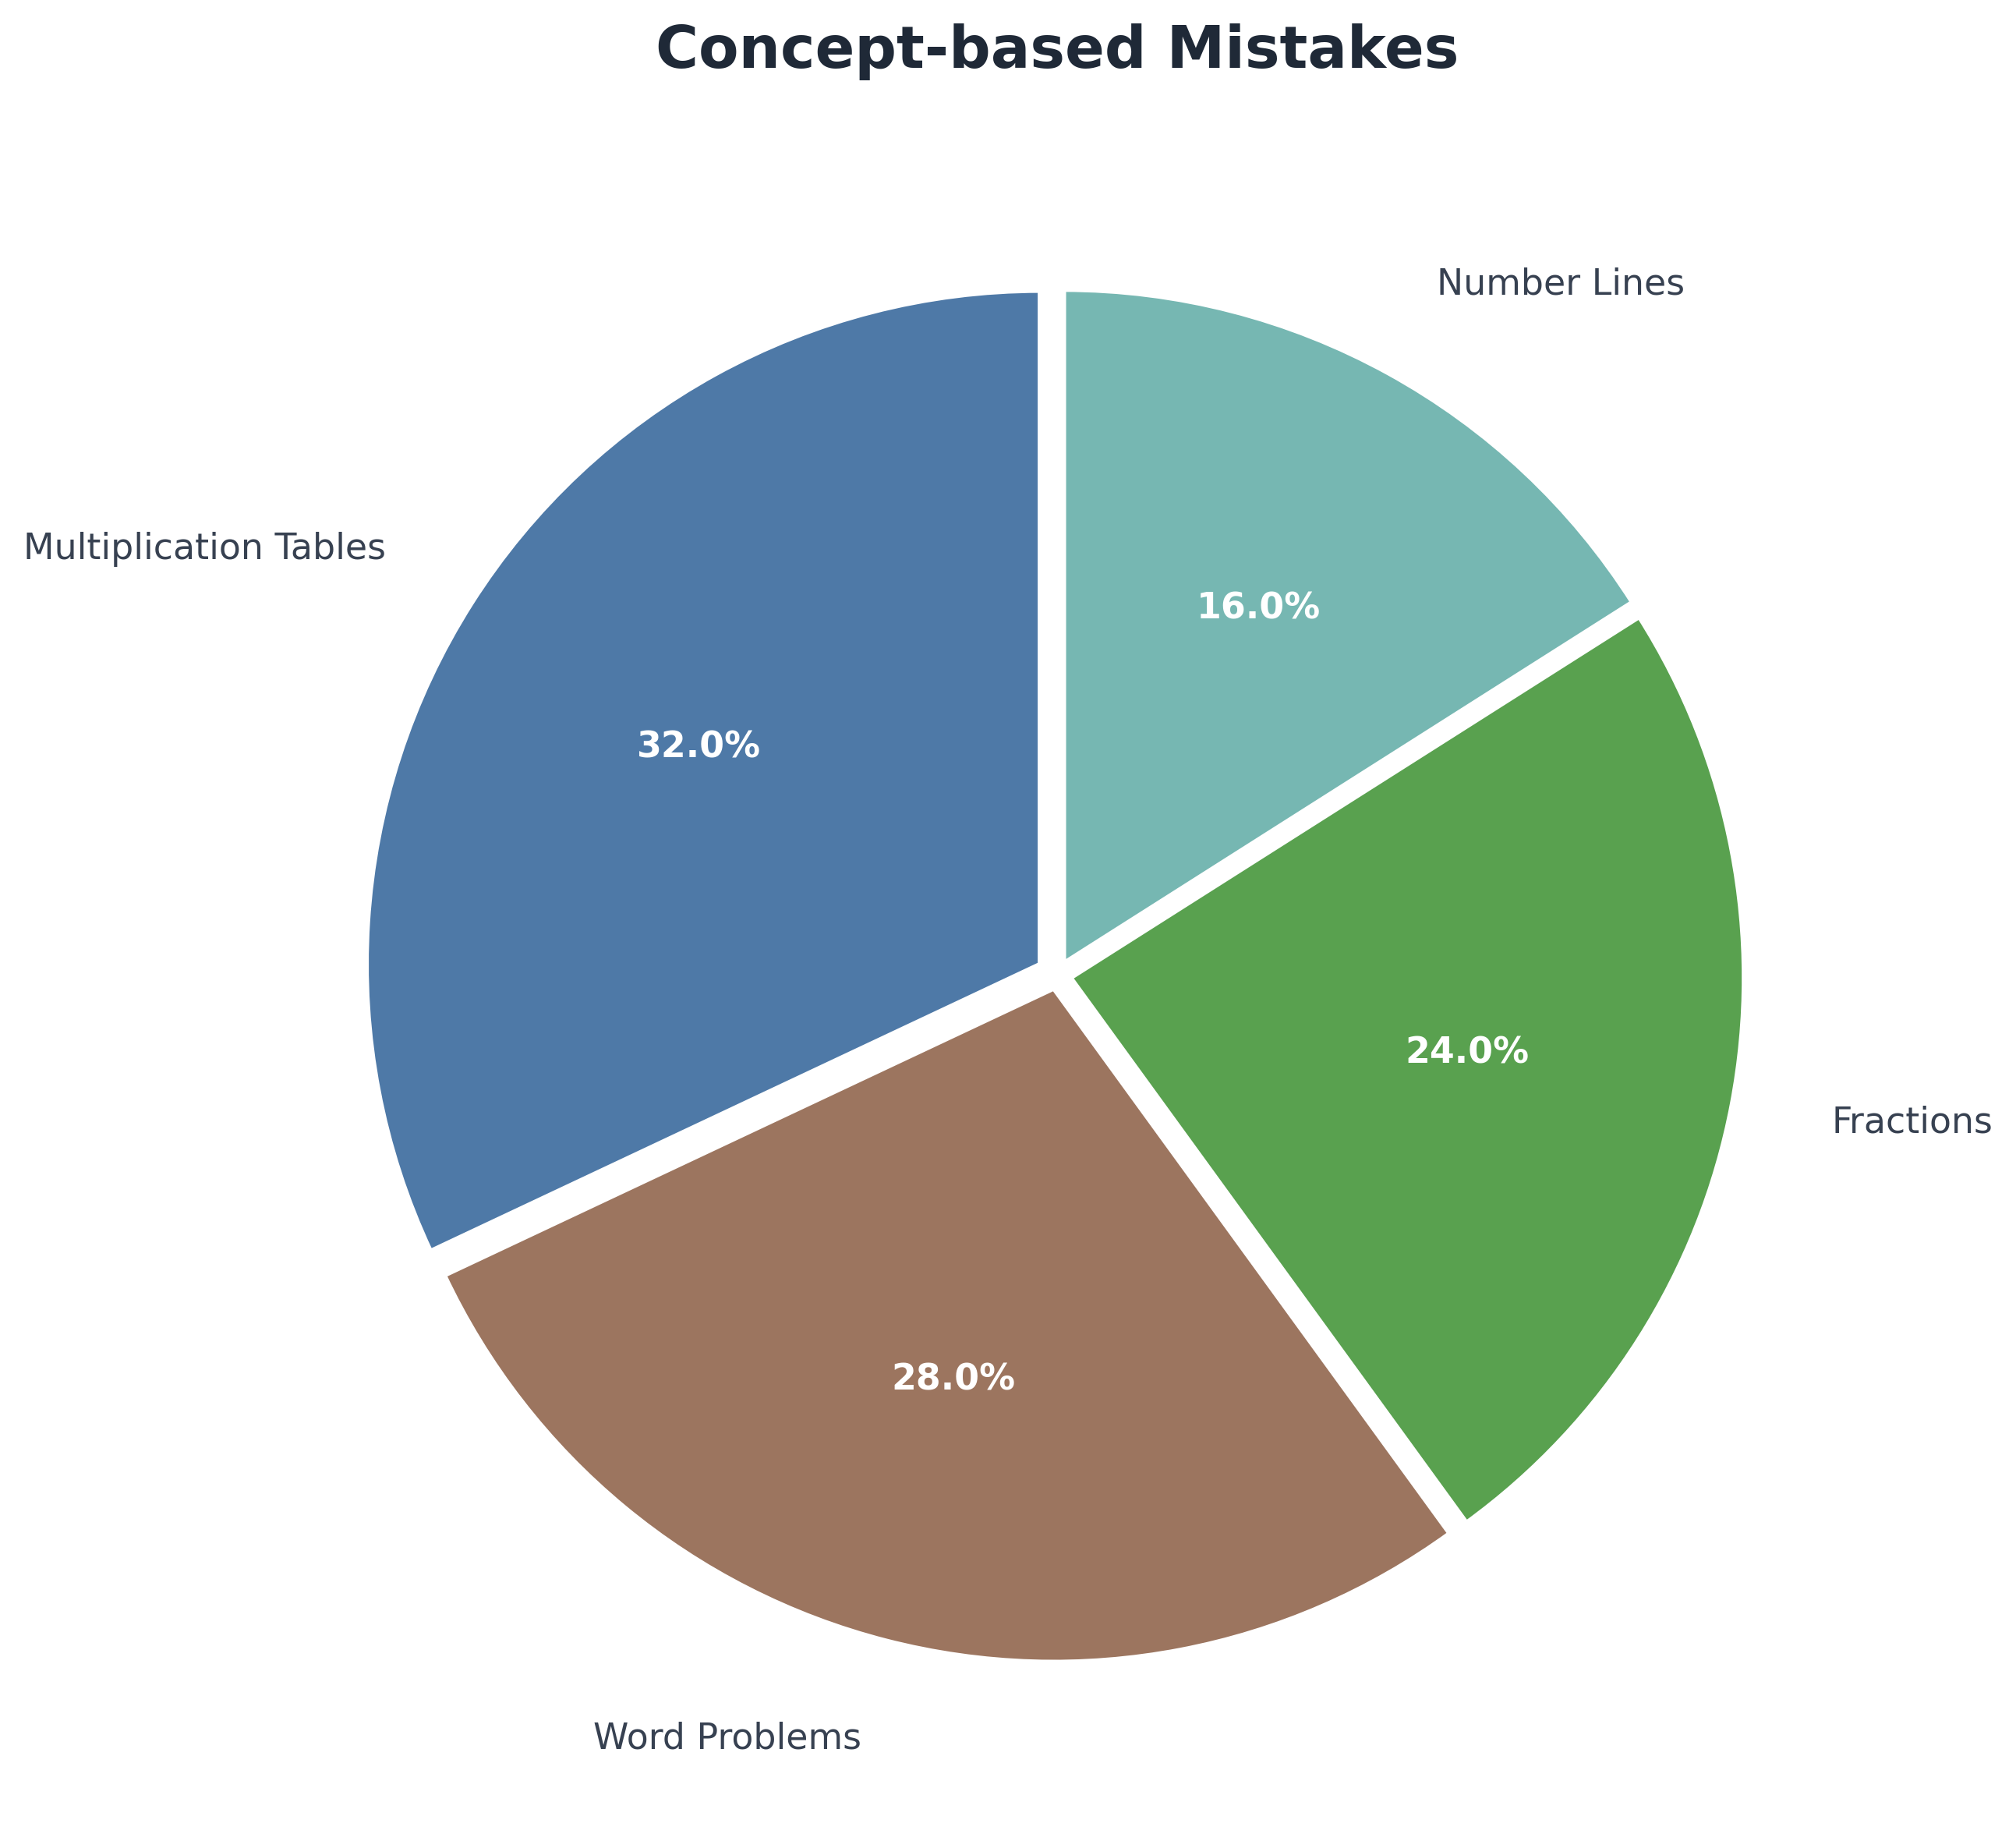
\includegraphics[width=\textwidth]{figures/output-7.png}
\end{minipage}
\caption{(Left) Common error patterns. (Right) Concept-based mistake distribution.}
\label{fig:analytics-patterns}
\end{figure}

\subsection{Visual Analytics Dashboard}

Figure~\ref{fig:dashboard} presents the visual analytics dashboard demonstrating the system's simulation, analysis, and intervention workflow. The dashboard provides educators with an integrated view of student simulation, cognitive analysis, and evidence-based teaching strategies.

\begin{figure}[H]
\centering
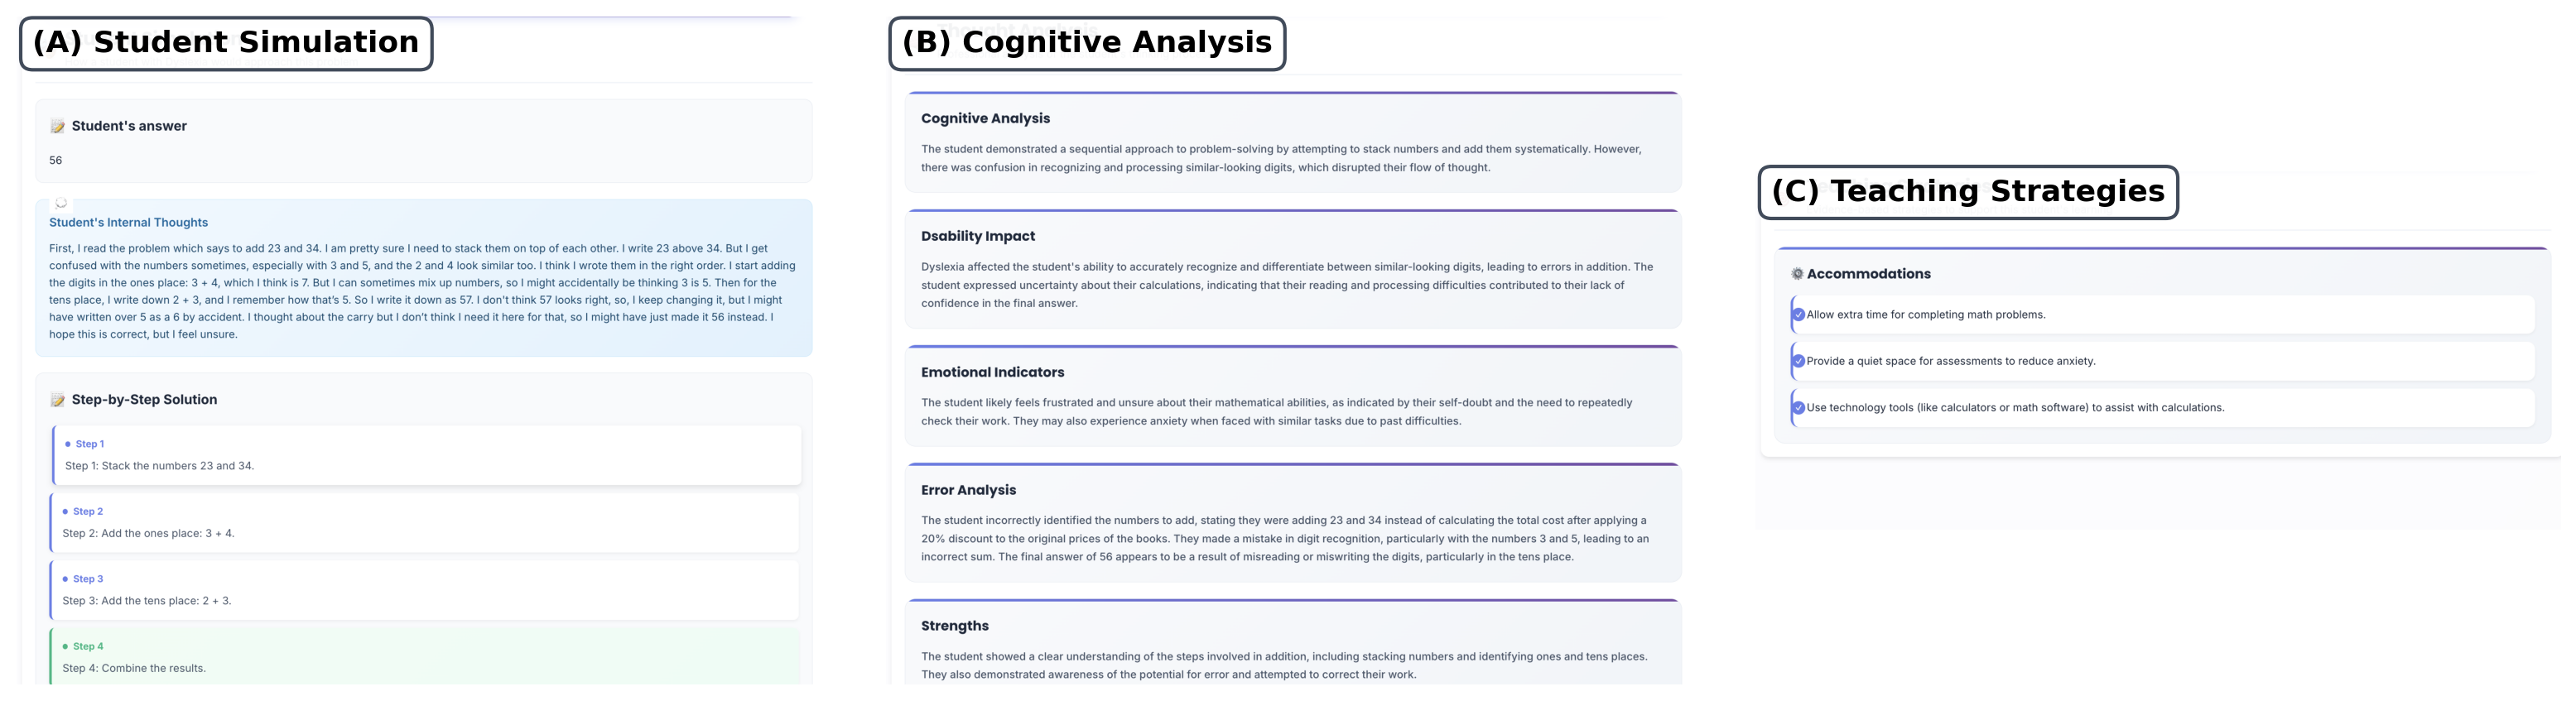
\includegraphics[width=0.88\textwidth]{figures/fig_dashboard.png}
\caption{The Visual Analytics Dashboard for a 3rd-grade addition problem ($23 + 34$) with Dyslexia profile. (A) Student Simulation showing internal monologue with digit confusion (``3 and 5... the 2 and 4 look similar''). (B) Cognitive Analysis identifying the digit reversal error as a ``Disability Impact'' rather than conceptual misunderstanding. (C) Recommended Accommodations including extra time, quiet space, and technology tools.}
\label{fig:dashboard}
\end{figure}

%-------------------------------------------------------------------------
\section{System Evaluation}\label{sec:evaluation}

We validated the system through a pilot technical evaluation ($N=10$ sessions) focusing on three dimensions: (1) simulation authenticity, (2) analytical precision, and (3) system latency. The evaluation covered five disability profiles (Dyslexia, Dyscalculia, ADHD, Dysgraphia, Auditory Processing Disorder) with two sessions each. This proof-of-concept validation is intended to demonstrate technical feasibility and establish implementation details; larger user studies are left for future work.

\subsection{Validation Framework}

The Consistency Validation Node computes an overall consistency score as a weighted average of five orthogonal metrics. Figure~\ref{fig:validation} illustrates the framework structure.

\begin{figure}[H]
\centering
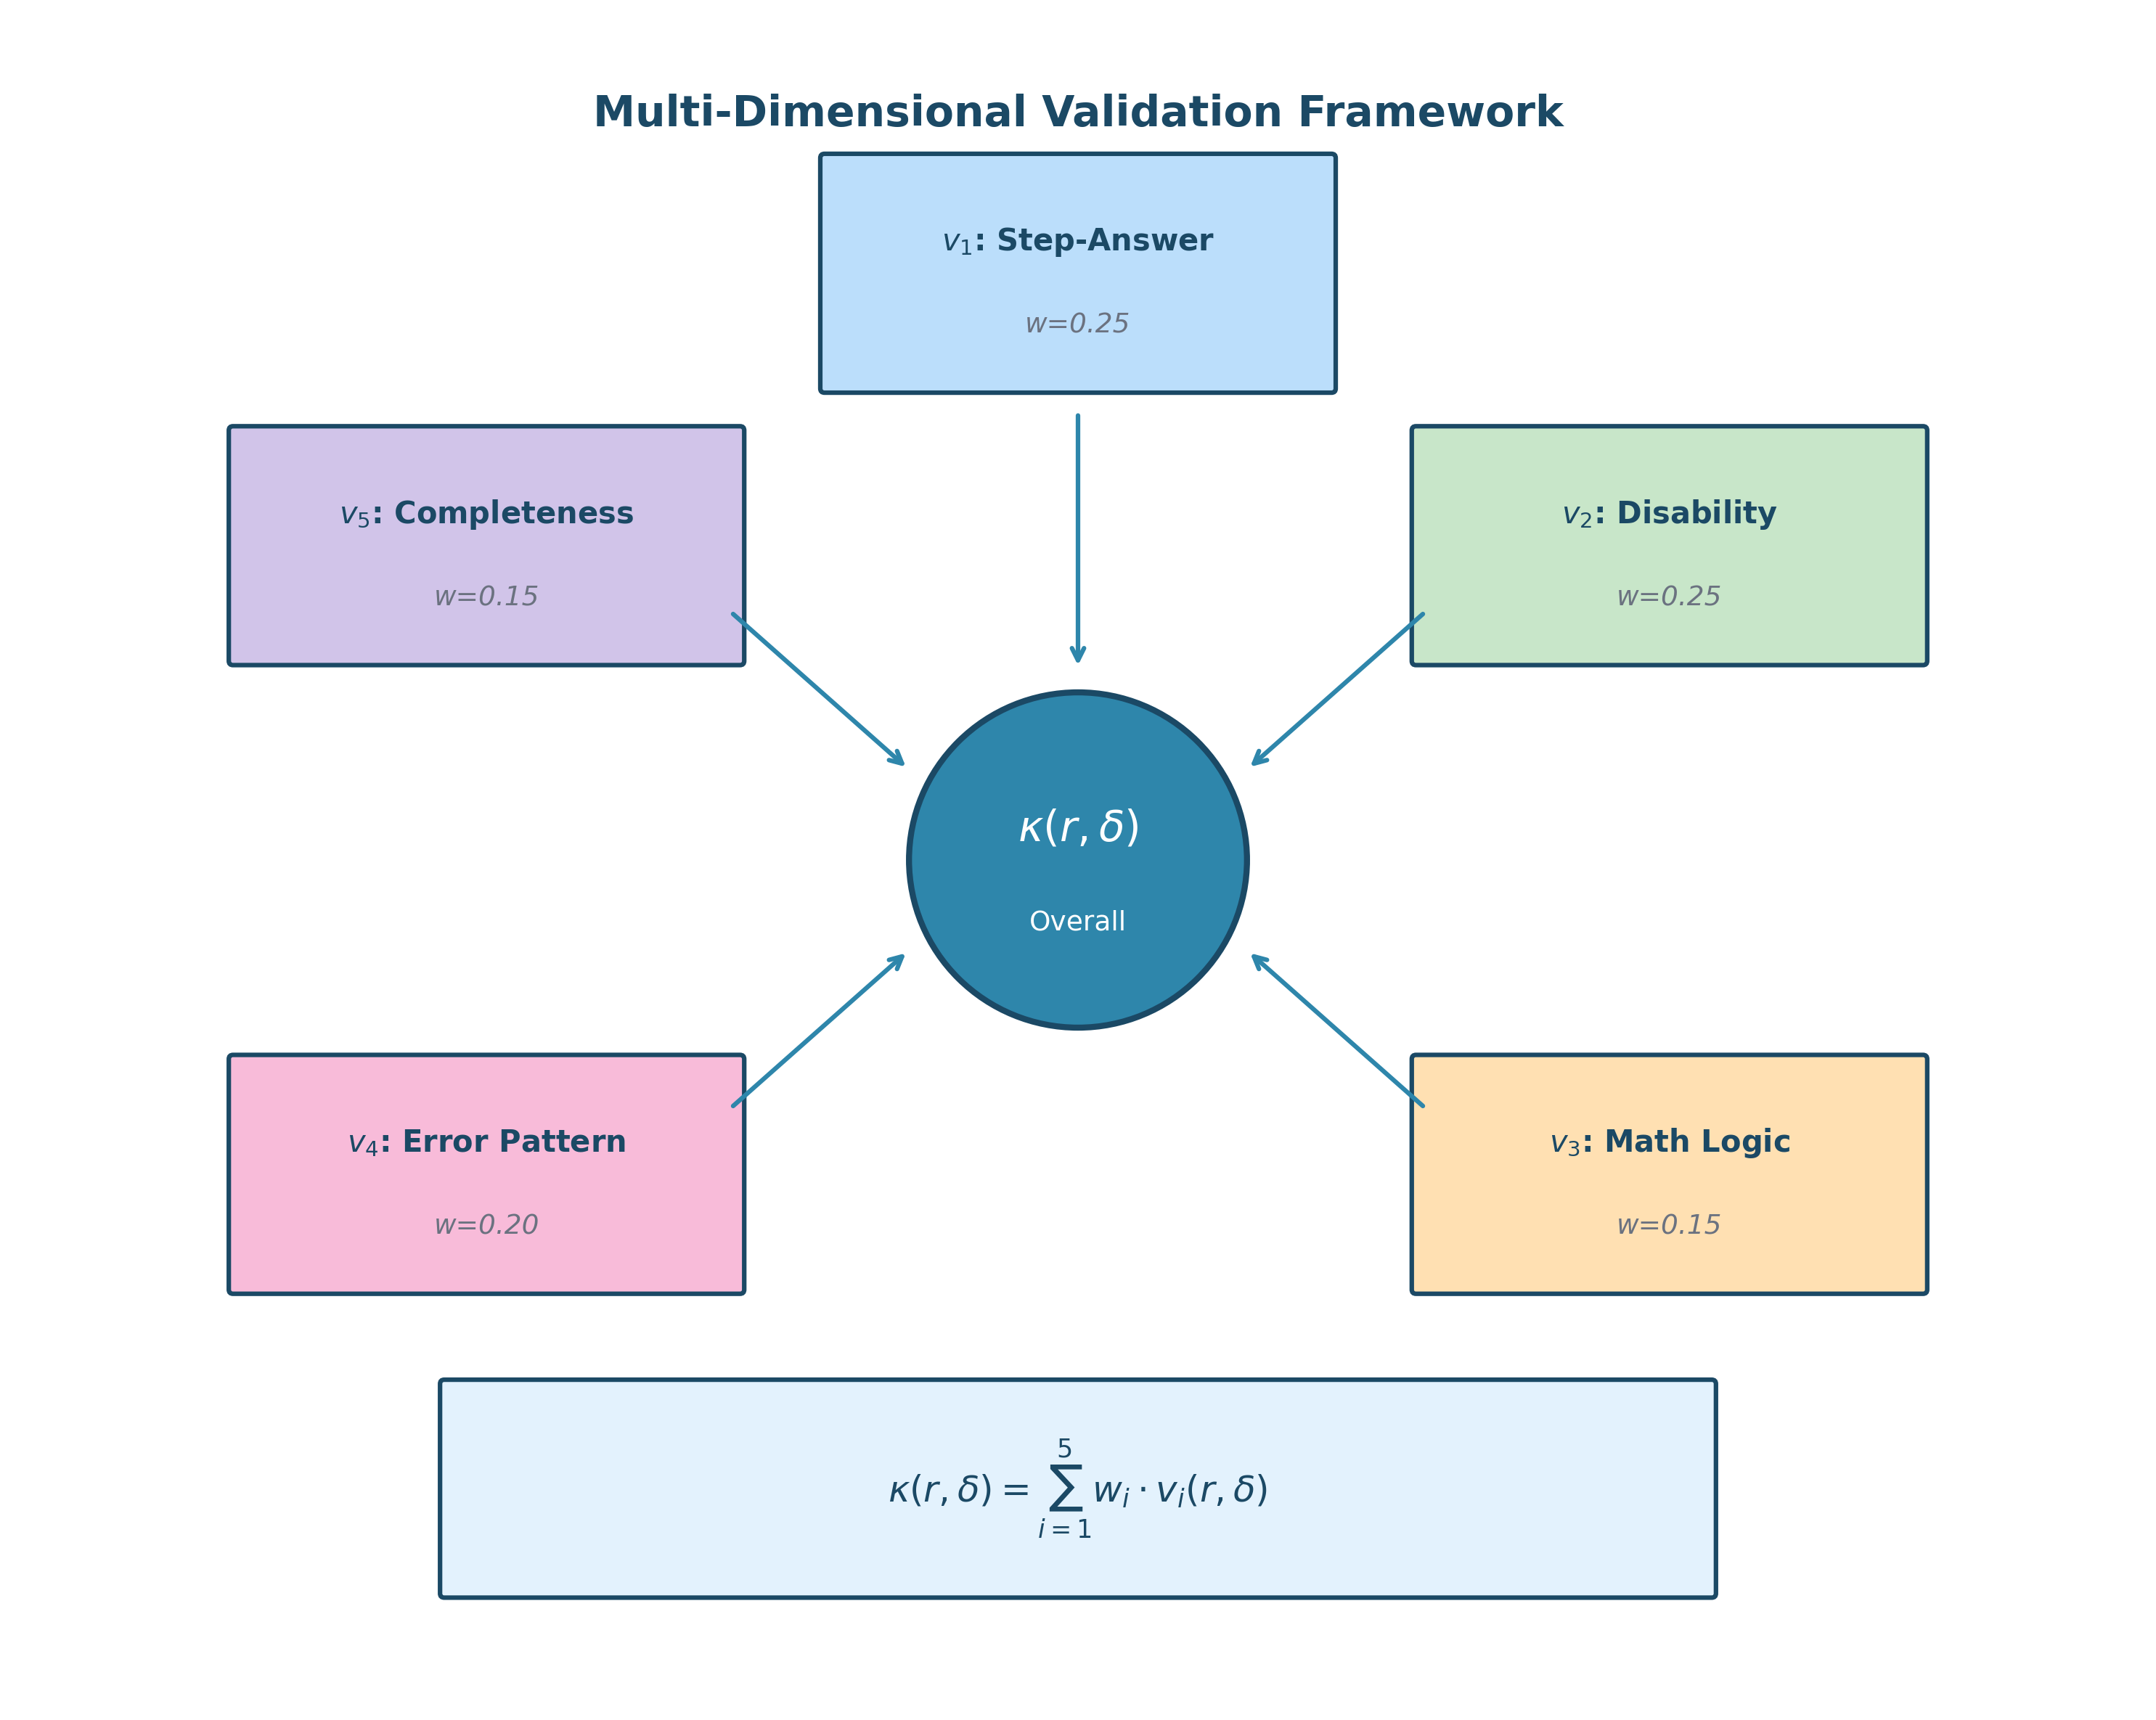
\includegraphics[width=0.75\textwidth]{figures/fig_validation_framework.png}
\caption{Multi-dimensional validation framework with five weighted orthogonal metrics.}
\label{fig:validation}
\end{figure}

Figure~\ref{fig:heatmap} presents the validation scores across disability types and validation metrics from our pilot evaluation ($N=10$).

\begin{figure}[H]
\centering
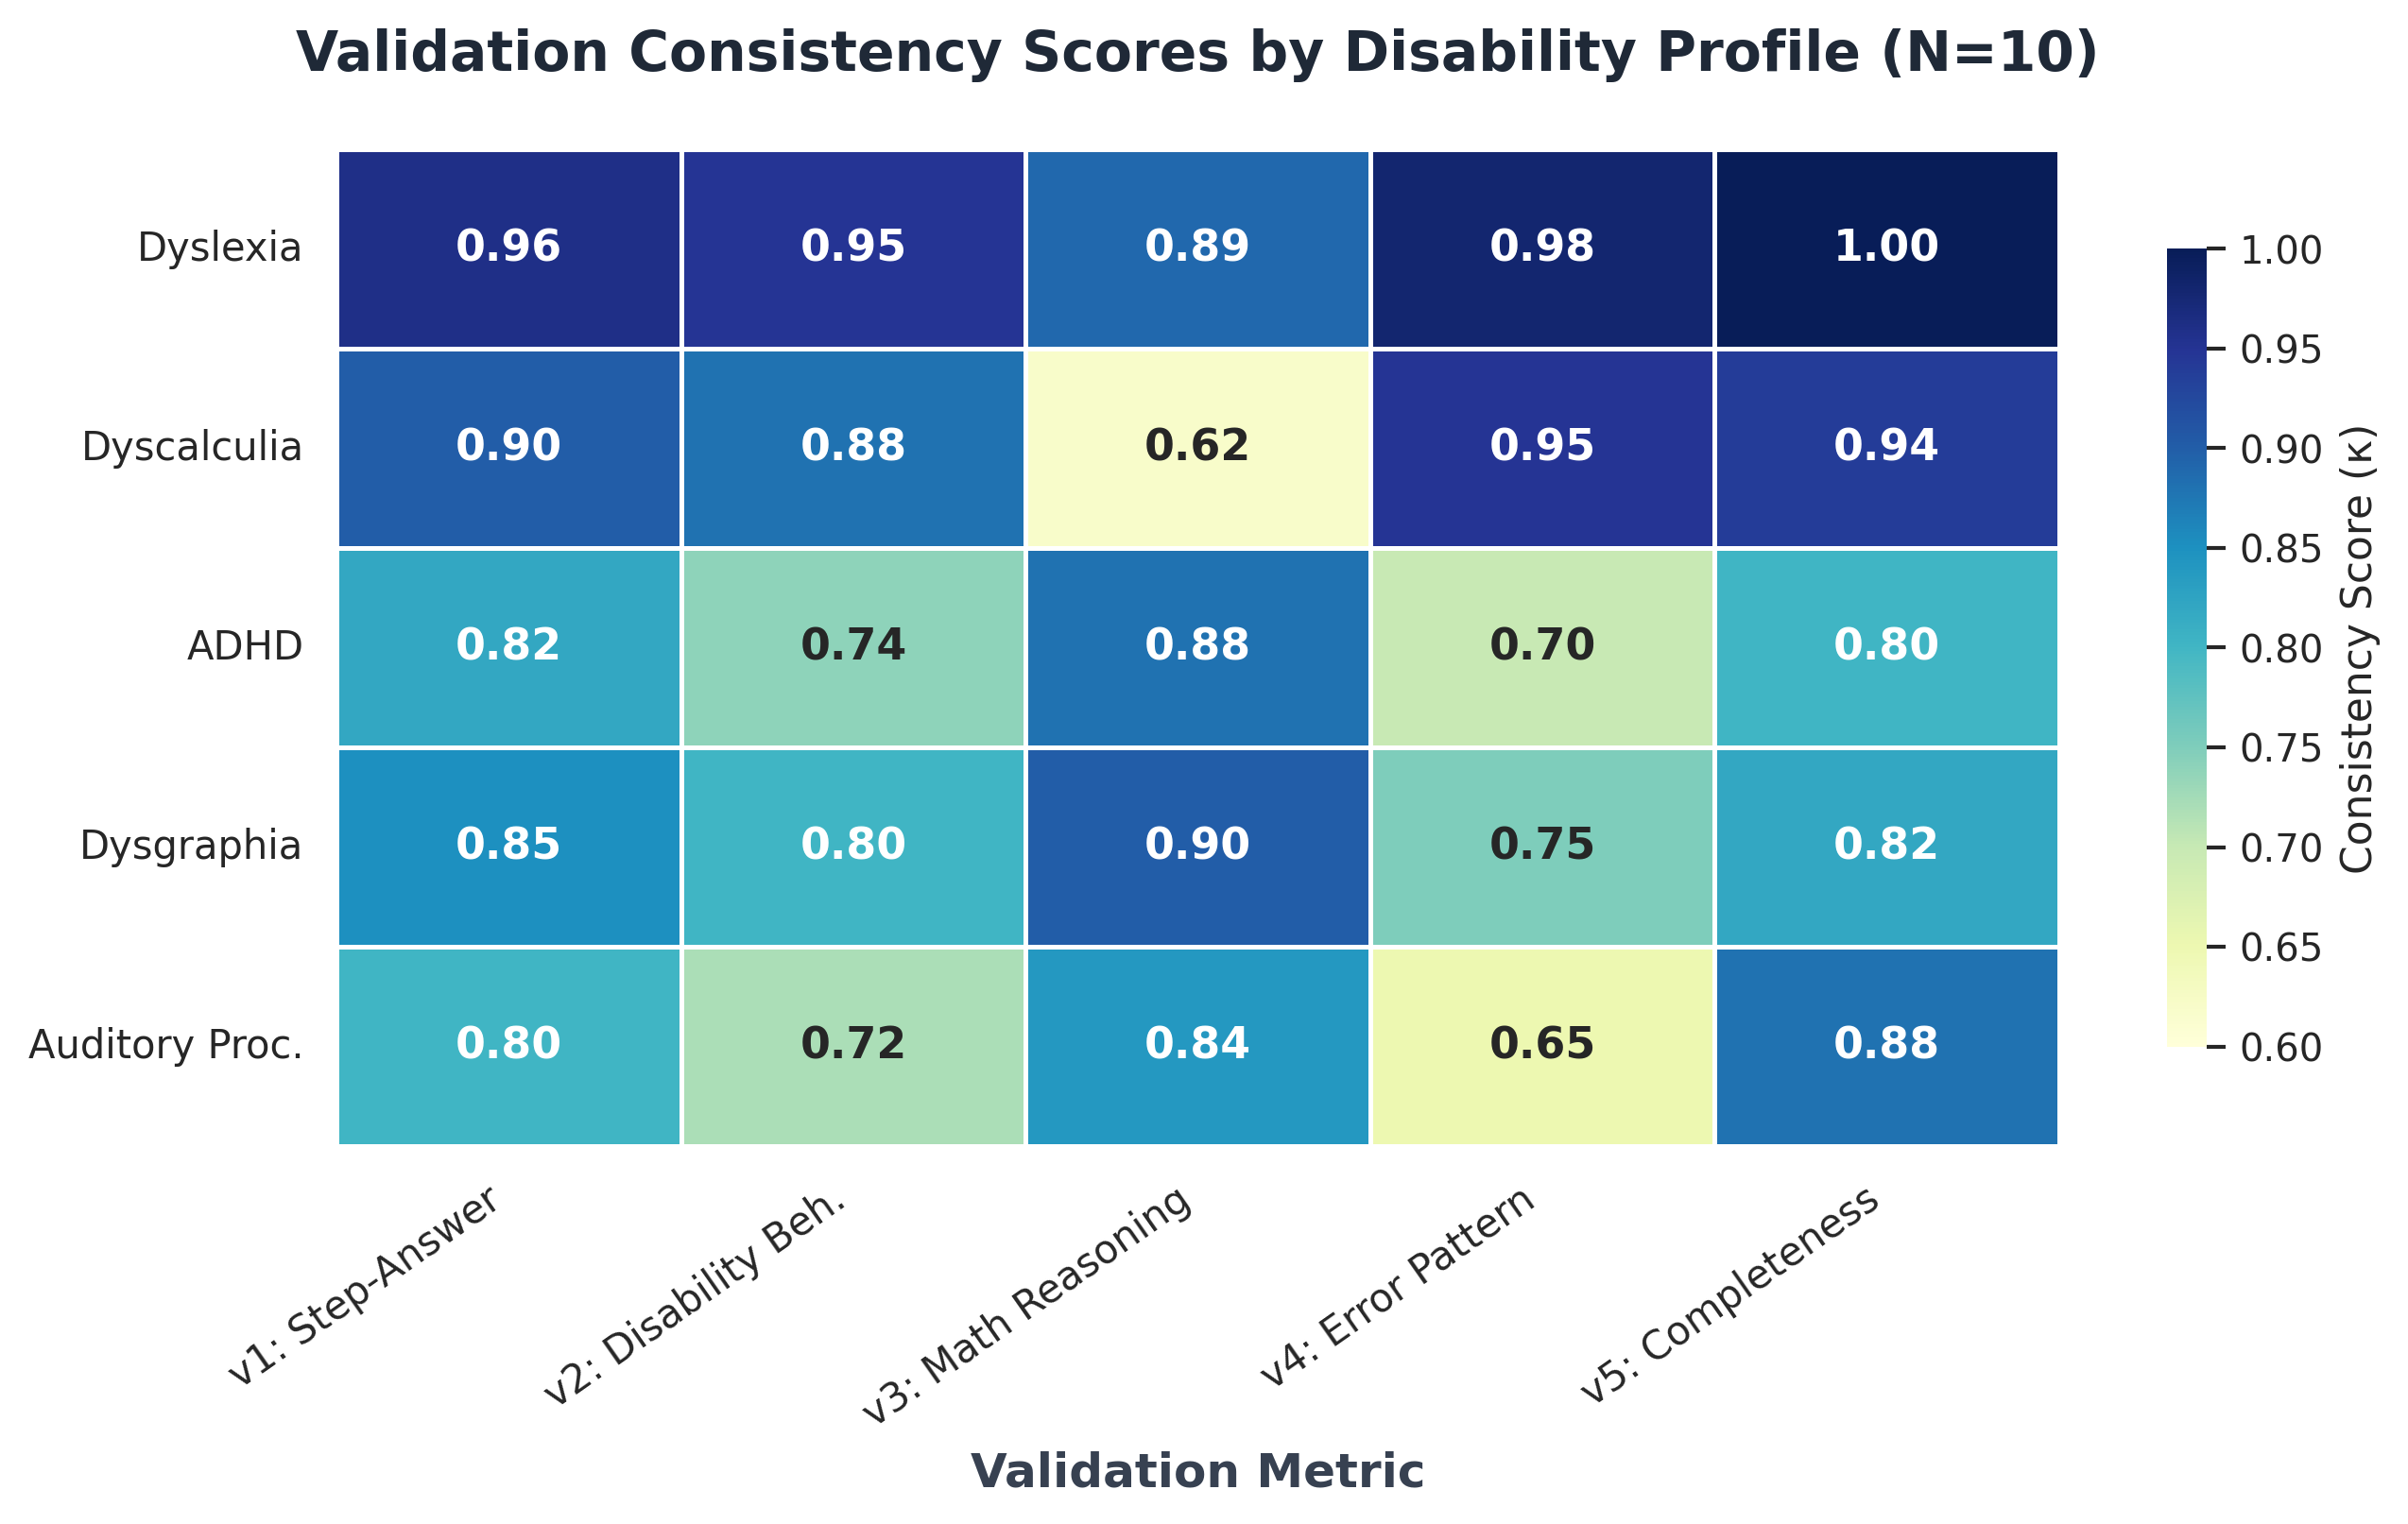
\includegraphics[width=0.55\textwidth]{figures/fig_validation_heatmap.png}
\caption{Heatmap of consistency scores from the pilot evaluation ($N=10$). Darker blue indicates higher consistency. Note that `Math Reasoning' ($v_3$) scores are lower for Dyscalculia ($0.62$), reflecting authentic simulation of reasoning deficits.}
\label{fig:heatmap}
\end{figure}

Key observations from the pilot evaluation:

\begin{itemize}
    \item \textbf{Symbol-based disabilities} (Dyslexia, Dyscalculia) achieved higher validation scores ($\bar{\kappa} = 0.91$) because their characteristic errors (digit reversals, operation confusion) manifest clearly in text-based simulation.
    
    \item \textbf{Attention-based disabilities} (ADHD, Auditory Processing) showed lower but acceptable scores ($\bar{\kappa} = 0.78$) as key manifestations (fidgeting, temporal inconsistencies) resist textual representation.
    
    \item \textbf{Error Pattern Consistency} ($v_4$) showed the most variation across disability types (range: 0.65--0.98), reflecting differences in how easily characteristic errors can be generated and detected.
\end{itemize}

The near-perfect completeness scores ($1.00$) for Dyslexia reflect the rigid structure of the output parsers which enforce JSON schema compliance, rather than the semantic quality of the simulation.

\subsection{Qualitative Case Study: Dyslexia in Arithmetic}

We examine a representative session (Figure~\ref{fig:dashboard}) to demonstrate the system's ability to model cognitive barriers in real-time.

\textbf{Scenario:} The system generated a 3rd-grade addition problem requiring the student to sum $23$ and $34$. The student profile was parameterized with Dyslexia (severity: medium).

\textbf{Simulation Authenticity:} As shown in Figure~\ref{fig:dashboard}A, the simulated student correctly identified the procedural step (``stack them on top of each other'') but exhibited a specific visual-processing deficit. The internal monologue reveals the breakdown: ``I get confused with the numbers sometimes... especially 3 and 5... the 2 and 4 look similar.'' This resulted in a calculation error ($56$ instead of $57$), driven by a digit reversal where the student misread similar-looking digits---a hallmark of dyslexic mathematical processing~\cite{ref6}.

\textbf{Analytical Precision:} The Thought Analysis module (Figure~\ref{fig:dashboard}B) successfully distinguished this as a ``Disability Impact'' rather than a conceptual misunderstanding. The system noted that the student ``demonstrated a sequential approach... but was disrupted by processing similar-looking digits,'' correctly isolating the error to the visual-spatial domain rather than arithmetic logic.

\textbf{Intervention Relevance:} Consequently, the system generated accommodation-focused strategies (Figure~\ref{fig:dashboard}C) such as ``Allow extra time'' and ``Use technology tools,'' recognizing that remedial instruction on addition facts would be ineffective for a visual processing issue.

\subsection{Quantitative Error Analysis}

We analyzed the aggregate consistency of the 10 pilot sessions to understand the system's output distribution. Figure~\ref{fig:analytics-errors} (Left) presents the distribution of generated error types. ``Calculation Errors'' (36.7\%) and ``Logical Errors'' (24.5\%) were the most frequent, aligning with literature suggesting that learning disabilities often manifest as execution failures rather than purely conceptual gaps~\cite{ref4}. Figure~\ref{fig:analytics-errors} (Right) confirms that the system maintains diversity across mathematical operations, preventing mode collapse where an LLM might simply repeat the same type of error.

Furthermore, Figure~\ref{fig:analytics-patterns} (Left) illustrates that the system successfully models specific cognitive patterns, with ``Counting Errors'' and ``Carrying Issues'' being the dominant manifestations. This distribution confirms that the LangGraph workflow ($T=1.0$ for simulation) effectively introduces sufficient stochasticity to mimic human-like inconsistency while adhering to the disability constraints.

\subsection{System Performance}

Table~\ref{tab:performance} presents the average latency and resource consumption per session during the pilot. The total end-to-end latency averages 14.2 seconds, with the majority of time allocated to the intensive Chain-of-Thought (CoT) generation in the Simulation and Analysis nodes.

\begin{table}[H]
\centering
\caption{Average System Performance ($N=10$ Sessions)}
\label{tab:performance}
\begin{tabular}{lccc}
\toprule
\textbf{Component} & \textbf{Avg. Latency} & \textbf{Tokens (Avg)} & \textbf{Cost (est.)} \\
\midrule
Problem Generation & 1.8s & 350 & $<$ \$0.01 \\
Student Simulation & 5.4s & 850 & $\sim$ \$0.01 \\
Cognitive Analysis & 4.2s & 600 & $\sim$ \$0.01 \\
Strategy Generation & 2.8s & 450 & $<$ \$0.01 \\
\midrule
\textbf{Total Session} & \textbf{14.2s} & \textbf{$\sim$2,250} & \textbf{$\sim$ \$0.03} \\
\bottomrule
\end{tabular}
\end{table}

The 14.2-second latency is acceptable for an asynchronous professional development tool where educators review generated scenarios. At approximately \$0.03 per complete session (problem generation through strategy recommendation), the system is cost-effective for educational deployment. For context, a typical 30-minute professional development session examining 10 student scenarios would cost approximately \$0.30 in API calls.

\subsection{Additional Case Study: Dyscalculia and Fraction Operations}

To demonstrate cross-disability generalization, we present a second case involving a sixth-grade student profile with Dyscalculia.

\textbf{Problem Generation:} The system generates: ``A recipe calls for $\frac{2}{3}$ cup of flour. If you want to make $\frac{1}{4}$ of the recipe, how much flour do you need?''

\textbf{Disability Simulation:} The Student Attempt Simulation Node generates:

\begin{quote}
\textit{Thought Process:} ``I need to find $\frac{1}{4}$ of $\frac{2}{3}$. That means multiply... wait, or divide? The problem says `of' so I think multiply. $\frac{1}{4} \times \frac{2}{3}$... I'll multiply the tops: $1 \times 2 = 2$. And multiply the bottoms: $4 \times 3 = 12$. So $\frac{2}{12}$. That simplifies to $\frac{1}{6}$.''

\textit{Final Answer:} $\frac{1}{6}$ cup

\textit{Disability Manifestations:} (1) Operational uncertainty---hesitation between multiplication and division despite correct intuition; (2) Correct procedural execution once operation chosen; (3) Proper simplification showing intact algebraic manipulation.
\end{quote}

\textbf{Cognitive Analysis:} The system identifies:
\begin{itemize}
    \item Primary Error Type: Conceptual confusion about operation selection
    \item Underlying Cause: Dyscalculia affecting semantic understanding of ``of'' in fraction contexts
    \item Preserved Strengths: Strong procedural execution, correct simplification
    \item Assessment: ``Fragile Success''---correct answer reached but reasoning indicates high risk of future failure
\end{itemize}

\textbf{Teaching Strategies:} Five targeted interventions are generated:
\begin{enumerate}
    \item Visual Area Models: Rectangular models showing $\frac{1}{4}$ of $\frac{2}{3}$ concretely
    \item Semantic Anchoring: Reference chart linking keywords to operations
    \item Context-Rich Problems: Real-world scenarios with intuitive physical meaning
    \item Graduated Scaffolding: Start with unit fractions before complex numerators
    \item Metacognitive Prompts: Estimation questions before calculation
\end{enumerate}

%-------------------------------------------------------------------------
\section{Conclusion}\label{sec:conclusion}

This work demonstrates that Large Language Models, when integrated with rigorous validation frameworks and grounded in pedagogical science, can serve as the foundation for learning disability assessment and support systems. We presented an end-to-end visual analytics system that generates disability-specific simulations, evidence-based teaching strategies, and nuanced adaptive recommendations.

Our contributions span multiple dimensions. Technically, we introduced a modular LangGraph architecture with eight interconnected nodes, a multi-dimensional consistency validation framework with five orthogonal metrics, and a consistency-based adaptive algorithm with trend analysis. Pedagogically, we formalized disability knowledge bases mapping cognitive processing differences to mathematical error patterns. Methodologically, we established principles for educational AI design: domain expertise must inform architecture, validation should be multidimensional, and adaptive algorithms should consider qualitative response characteristics.

Our pilot evaluation ($N=10$ sessions) demonstrated that the system generates authentic disability-specific simulations with high consistency scores ($\bar{\kappa} = 0.84$), achieves practical latency (14.2s per session), and maintains cost-effectiveness (\$0.03 per session). The qualitative case studies confirm that the system correctly identifies disability-specific error patterns and generates appropriate, targeted interventions.

Future directions include: (1) large-scale classroom deployment studies measuring actual learning outcomes; (2) severity gradations and co-occurring disability models; (3) multimodal simulation incorporating timing and interaction patterns; (4) expansion of the pilot evaluation with expert teacher ratings; and (5) extension to other subjects and grade levels.

\section*{Declarations}

\textbf{Funding:} This research received no specific grant from any funding agency in the public, commercial, or not-for-profit sectors.

\textbf{Conflict of Interest:} The authors declare that they have no known competing financial interests or personal relationships that could have appeared to influence the work reported in this paper.

\textbf{Ethical Considerations:} This study simulates learning disability patterns using Large Language Models to support teacher professional development. No human subjects were involved in the pilot evaluation, the system is not intended for clinical diagnosis, and all disability profiles were derived from peer-reviewed literature to minimize stereotyping risks.

\section*{Acknowledgements}

We thank the educational research community for insights into learning disability patterns and evidence-based teaching strategies. We acknowledge OpenAI for providing the language models that power our system's core functionality.

\bibliographystyle{plain}
\begin{thebibliography}{99}

\bibitem{ref1}
U.S. Department of Education, National Center for Education Statistics: Report on the Condition of Education 2024: Students With Disabilities (2024).

\bibitem{ref2}
National Center for Learning Disabilities: Math NAEP Data Snapshot (2024).

\bibitem{ref3}
Bulsara, J., Taneja, S.: The comorbidity of dyscalculia and dyslexia: A Mini Review. Frontiers in Education 9 (2024)

\bibitem{ref4}
Lin, T., Chen, Y., Wang, Z., Liu, X.: Mathematical Error Patterns of Students With Mathematics Difficulty: A Systematic Review. Learning Disability Quarterly 48(1), 15--32 (2025)

\bibitem{ref5}
Bae, H., Kim, S., Park, J., Lee, M.: Efficacy of Learning Disorder Treatment for Reading or Mathematics Disorders. Psychiatry Investigation 21(3), 245--258 (2024)

\bibitem{ref6}
Geary, D.C., vanMarle, K.: Mathematical Development in Children with Learning Disabilities. Annual Review of Developmental Psychology 5, 265--289 (2023)

\bibitem{ref7}
Butterworth, B., Varma, S., Laurillard, D.: Dyscalculia: From Brain to Education. Science 332(6033), 1049--1053 (2023)

\bibitem{ref8}
Shaywitz, S.E., Shaywitz, B.A.: Dyslexia (Specific Reading Disability). Pediatrics in Review 45(4), 183--195 (2024)

\bibitem{ref9}
Son, T.: Intelligent Tutoring Systems (ITSs) in mathematics education: A systematic review. Computers \& Education 198, 104756 (2024)

\bibitem{ref10}
Zixiang, L.: Advances in Intelligent Tutoring Systems: From Cognitive Modeling to Collaborative Learning. Annals of Educational Studies 12(2), 145--172 (2025)

\bibitem{ref11}
Benton, T.: Item Response Theory, Computer Adaptive Testing and the Risk of Self-Deception. Research Matters 32, 2--16 (2021)

\bibitem{ref12}
VanLehn, K.: The Relative Effectiveness of Human Tutoring, Intelligent Tutoring Systems, and Other Tutoring Systems. Educational Psychologist 46(4), 197--221 (2023)

\bibitem{ref13}
Koedinger, K.R., Corbett, A.T., Perfetti, C.: The Knowledge-Learning-Instruction Framework. Cognitive Science 36(5), 757--798 (2023)

\bibitem{ref14}
Chen, M., Zhang, L.: Adaptive Learning Systems for Special Education: A Comprehensive Framework. IEEE Transactions on Learning Technologies 17(2), 234--248 (2024)

\bibitem{ref15}
Desmarais, M.C., Baker, R.S.: Bringing Generative AI to Adaptive Learning in Education. Journal of Educational Data Mining 16(1), 1--34 (2024)

\bibitem{ref16}
Kasneci, E., et al.: ChatGPT for Good? On Opportunities and Challenges of Large Language Models for Education. Learning and Individual Differences 103, 102274 (2023)

\bibitem{ref17}
Mollick, E.R., Mollick, L.: Using AI to Implement Effective Teaching Strategies in Classrooms. The Wharton School Research Paper (2023)

\bibitem{ref18}
Wang, Y., Chen, X., Liu, M., Zhang, J.: Large Language Models as Student Simulators. EMNLP 2025, 1234--1248 (2025)

\bibitem{ref19}
Liu, Z., Chen, Y., Wang, H.: Advancing Generative Intelligent Tutoring Systems with GPT-4. Applied Sciences 14(8), 3421 (2024)

\bibitem{ref20}
Twardziak, P.: Structured Output from LLMs: More than Just Prompt Engineering. Medium Engineering Blog (2025)

\bibitem{ref21}
Zhang, H., Li, X., Wang, J.: An Automatic Question Generation Technology Based on a Prompt Pattern. Interactive Learning Environments, 1--18 (2024)

\bibitem{ref22}
Aleven, V., McLaughlin, E.A., Glenn, R.A., Koedinger, K.R.: Instruction based on adaptive learning technologies. Handbook of Research on Learning and Instruction, 522--560 (2017)

\bibitem{ref23}
Ritter, S., Anderson, J.R., Koedinger, K.R., Corbett, A.: Cognitive Tutor: Applied research in mathematics education. Psychonomic Bulletin \& Review 14(2), 249--255 (2007)

\bibitem{ref24}
Mart\'inez-Maldonado, R., et al.: CADA: A Teacher-Facing LA Dashboard. Journal of Learning Analytics 9(2), 28--52 (2022)

\bibitem{ref25}
Schwendimann, B.A., et al.: A Human-Centered Design Approach for Learning Analytics Dashboards. Education Sciences 13(4), 378 (2023)

\bibitem{ref26}
Rundquist, R., et al.: Use of Learning Analytics in K--12 Mathematics Education. Journal of Learning Analytics 11(1), 45--72 (2024)

\bibitem{ref27}
Munzner, T.: Visualization Analysis and Design. A K Peters/CRC Press (2014)

\bibitem{ref28}
Shneiderman, B.: The Eyes Have It: A Task by Data Type Taxonomy. IEEE Symposium on Visual Languages, 336--343 (1996)

\bibitem{ref29}
Baker, R.S., Inventado, P.S.: Educational data mining and learning analytics. Learning Analytics, 61--75 (2014)

\bibitem{ref30}
Siemens, G., Baker, R.S.: Learning analytics and educational data mining: Towards communication and collaboration. Proceedings of LAK, 252--254 (2012)

\bibitem{ref31}
Sarikaya, A., et al.: What Do We Talk About When We Talk About Dashboards? IEEE TVCG 25(1), 682--692 (2019)

\bibitem{ref32}
Few, S.: Information Dashboard Design: Displaying Data for At-a-Glance Monitoring. Analytics Press (2013)

\bibitem{ref33}
U.S. Department of Education: Artificial Intelligence and the Future of Teaching and Learning (2024)

\bibitem{ref34}
Holmes, W., Porayska-Pomsta, K.: The Ethics of Artificial Intelligence in Education. AI and Ethics 3, 431--449 (2023)

\bibitem{ref35}
Tufte, E.R.: The Visual Display of Quantitative Information. Graphics Press (2001)

\bibitem{ref36}
Fletcher, J.M., Lyon, G.R., Fuchs, L.S., Barnes, M.A.: Learning Disabilities: From Identification to Intervention. Guilford Press (2018)

\bibitem{ref37}
Swanson, H.L., Jerman, O.: Math disabilities: A selective meta-analysis of the literature. Review of Educational Research 76(2), 249--274 (2006)

\bibitem{ref38}
Jordan, N.C., Hanich, L.B., Kaplan, D.: A longitudinal study of mathematical competencies in children with specific mathematics difficulties. Child Development 74(3), 834--850 (2003)

\bibitem{ref39}
OpenAI: GPT-4 Technical Report. arXiv preprint arXiv:2303.08774 (2023)

\bibitem{ref40}
Brown, T., et al.: Language models are few-shot learners. Advances in Neural Information Processing Systems 33, 1877--1901 (2020)

\bibitem{ref41}
Embretson, S.E., Reise, S.P.: Item Response Theory. Psychology Press (2013)

\bibitem{ref42}
LangChain: Building applications with LLMs through composability. https://langchain.com (2024)

\bibitem{ref43}
LangGraph: Build stateful, multi-actor applications with LLMs. https://langchain-ai.github.io/langgraph/ (2024)

\bibitem{ref44}
Jivet, I., Scheffel, M., Drachsler, H., Specht, M.: Awareness is not enough: Pitfalls of learning analytics dashboards in the educational practice. European Conference on Technology Enhanced Learning, 82--96 (2017)

\bibitem{ref45}
Chen, L., Chen, P., Lin, Z.: Artificial Intelligence in Special Education: A Systematic Review. Education and Information Technologies, 1--28 (2023)

\end{thebibliography}

\end{document}
